% Options for packages loaded elsewhere
\PassOptionsToPackage{unicode}{hyperref}
\PassOptionsToPackage{hyphens}{url}
\PassOptionsToPackage{dvipsnames,svgnames,x11names}{xcolor}
%
\documentclass[
  12pt,
  authoryear,
  preprint,
  3p]{elsarticle}

\usepackage{amsmath,amssymb}
\usepackage{iftex}
\ifPDFTeX
  \usepackage[T1]{fontenc}
  \usepackage[utf8]{inputenc}
  \usepackage{textcomp} % provide euro and other symbols
\else % if luatex or xetex
  \usepackage{unicode-math}
  \defaultfontfeatures{Scale=MatchLowercase}
  \defaultfontfeatures[\rmfamily]{Ligatures=TeX,Scale=1}
\fi
\usepackage{lmodern}
\ifPDFTeX\else  
    % xetex/luatex font selection
\fi
% Use upquote if available, for straight quotes in verbatim environments
\IfFileExists{upquote.sty}{\usepackage{upquote}}{}
\IfFileExists{microtype.sty}{% use microtype if available
  \usepackage[]{microtype}
  \UseMicrotypeSet[protrusion]{basicmath} % disable protrusion for tt fonts
}{}
\makeatletter
\@ifundefined{KOMAClassName}{% if non-KOMA class
  \IfFileExists{parskip.sty}{%
    \usepackage{parskip}
  }{% else
    \setlength{\parindent}{0pt}
    \setlength{\parskip}{6pt plus 2pt minus 1pt}}
}{% if KOMA class
  \KOMAoptions{parskip=half}}
\makeatother
\usepackage{xcolor}
\setlength{\emergencystretch}{3em} % prevent overfull lines
\setcounter{secnumdepth}{5}
% Make \paragraph and \subparagraph free-standing
\ifx\paragraph\undefined\else
  \let\oldparagraph\paragraph
  \renewcommand{\paragraph}[1]{\oldparagraph{#1}\mbox{}}
\fi
\ifx\subparagraph\undefined\else
  \let\oldsubparagraph\subparagraph
  \renewcommand{\subparagraph}[1]{\oldsubparagraph{#1}\mbox{}}
\fi


\providecommand{\tightlist}{%
  \setlength{\itemsep}{0pt}\setlength{\parskip}{0pt}}\usepackage{longtable,booktabs,array}
\usepackage{calc} % for calculating minipage widths
% Correct order of tables after \paragraph or \subparagraph
\usepackage{etoolbox}
\makeatletter
\patchcmd\longtable{\par}{\if@noskipsec\mbox{}\fi\par}{}{}
\makeatother
% Allow footnotes in longtable head/foot
\IfFileExists{footnotehyper.sty}{\usepackage{footnotehyper}}{\usepackage{footnote}}
\makesavenoteenv{longtable}
\usepackage{graphicx}
\makeatletter
\def\maxwidth{\ifdim\Gin@nat@width>\linewidth\linewidth\else\Gin@nat@width\fi}
\def\maxheight{\ifdim\Gin@nat@height>\textheight\textheight\else\Gin@nat@height\fi}
\makeatother
% Scale images if necessary, so that they will not overflow the page
% margins by default, and it is still possible to overwrite the defaults
% using explicit options in \includegraphics[width, height, ...]{}
\setkeys{Gin}{width=\maxwidth,height=\maxheight,keepaspectratio}
% Set default figure placement to htbp
\makeatletter
\def\fps@figure{htbp}
\makeatother

\usepackage{booktabs}
\usepackage{longtable}
\usepackage{array}
\usepackage{multirow}
\usepackage{wrapfig}
\usepackage{float}
\usepackage{colortbl}
\usepackage{pdflscape}
\usepackage{tabu}
\usepackage{threeparttable}
\usepackage{threeparttablex}
\usepackage[normalem]{ulem}
\usepackage{makecell}
\usepackage{xcolor}
\usepackage{placeins}
\usepackage{setspace}
\usepackage{lineno}
\onehalfspacing
\linespread{2}
\linenumbers
\makeatletter
\makeatother
\makeatletter
\makeatother
\makeatletter
\@ifpackageloaded{caption}{}{\usepackage{caption}}
\AtBeginDocument{%
\ifdefined\contentsname
  \renewcommand*\contentsname{Table of contents}
\else
  \newcommand\contentsname{Table of contents}
\fi
\ifdefined\listfigurename
  \renewcommand*\listfigurename{List of Figures}
\else
  \newcommand\listfigurename{List of Figures}
\fi
\ifdefined\listtablename
  \renewcommand*\listtablename{List of Tables}
\else
  \newcommand\listtablename{List of Tables}
\fi
\ifdefined\figurename
  \renewcommand*\figurename{Figure}
\else
  \newcommand\figurename{Figure}
\fi
\ifdefined\tablename
  \renewcommand*\tablename{Table}
\else
  \newcommand\tablename{Table}
\fi
}
\@ifpackageloaded{float}{}{\usepackage{float}}
\floatstyle{ruled}
\@ifundefined{c@chapter}{\newfloat{codelisting}{h}{lop}}{\newfloat{codelisting}{h}{lop}[chapter]}
\floatname{codelisting}{Listing}
\newcommand*\listoflistings{\listof{codelisting}{List of Listings}}
\makeatother
\makeatletter
\@ifpackageloaded{caption}{}{\usepackage{caption}}
\@ifpackageloaded{subcaption}{}{\usepackage{subcaption}}
\makeatother
\makeatletter
\@ifpackageloaded{tcolorbox}{}{\usepackage[skins,breakable]{tcolorbox}}
\makeatother
\makeatletter
\@ifundefined{shadecolor}{\definecolor{shadecolor}{rgb}{.97, .97, .97}}
\makeatother
\makeatletter
\makeatother
\makeatletter
\makeatother
\journal{Fisheries Research}
\ifLuaTeX
  \usepackage{selnolig}  % disable illegal ligatures
\fi
\usepackage[]{natbib}
\bibliographystyle{elsarticle-harv}
\IfFileExists{bookmark.sty}{\usepackage{bookmark}}{\usepackage{hyperref}}
\IfFileExists{xurl.sty}{\usepackage{xurl}}{} % add URL line breaks if available
\urlstyle{same} % disable monospaced font for URLs
\hypersetup{
  pdftitle={Methods to incorporate known habitat in indices of abundance for rocky reef associated species and applications to management},
  pdfauthor={Melissa Hedges Monk; Rebecca R. Miller; E.J. Dick; Grant Waltz; Dean Wendt},
  pdfkeywords={fisheries dependent data, habitat
association, groundfish, index of abundance},
  colorlinks=true,
  linkcolor={blue},
  filecolor={Maroon},
  citecolor={Blue},
  urlcolor={Blue},
  pdfcreator={LaTeX via pandoc}}

\setlength{\parindent}{6pt}
\begin{document}

\begin{frontmatter}
\title{Methods to incorporate known habitat in indices of abundance for
rocky reef associated species and applications to management}
\author[1]{Melissa Hedges Monk%
\corref{cor1}%
\fnref{fn1}}
 \ead{melissa.monk@noaa.gov} 
\author[2]{Rebecca R. Miller%
%
}
 \ead{rebecca.miller@noaa.gov} 
\author[1]{E.J. Dick%
%
}
 \ead{edward.dick@noaa.gov} 
\author[33]{Grant Waltz%
%
}
 \ead{cat@example.com} 
\author[3]{Dean Wendt%
%
}
 \ead{cat@example.com} 

\affiliation[1]{organization={Southwest Fisheries Science
Center}, addressline={110 McAllister Way}, city={Santa
Cruz}, country={}, postcode={95060}}

\affiliation[2]{organization={University of California Santa
Cruz}, addressline={Street Address}, city={Santa
Cruz}, country={}, postcode={95060}}

\affiliation[3]{organization={California Polytechnic State
University}, addressline={Street Address}, city={San Luis
Obispo}, country={}, postcode={93407}}


\cortext[cor1]{Corresponding author}
\fntext[fn1]{This is the first author footnote.}




        
\begin{abstract}
Indices of abundance developed from fishery-dependent data are typically
subject to a number of assumptions about the area and habitat fished due
to the aggregation of the catch at the level of a fishing trip.

In California, two surveys occur onboard the recreational charter boats
fleet and samplers record location-specific data on the catch and effort
during individual fishing stops throughout a trip. This location
specific information coupled with high-resolution maps of the bottom
substrate allowed us to subset the survey data to areas of rocky reef
habitat. The six species of rockfish (\emph{Sebastes} spp.) modeled in
this paper as example all have high affinity to rocky habitat. We
compared the indices of abundance developed with and without including
information on rocky reef habitat. The identification of the rocky reefs
also allowed us to weight the index of abundance by the area of
available habitat with predefined regions. We show that in general the
finer scale trends are variable and weighting the indices by the amount
of habitat within finer scale area decrease the variance around the
estimates. We also show how the estimates of available habitat can be
used to portion catches across management areas.
\end{abstract}





\begin{keyword}
    fisheries dependent data \sep habitat
association \sep groundfish \sep 
    index of abundance
\end{keyword}
\end{frontmatter}\ifdefined\Shaded\renewenvironment{Shaded}{\begin{tcolorbox}[borderline west={3pt}{0pt}{shadecolor}, interior hidden, enhanced, boxrule=0pt, frame hidden, sharp corners, breakable]}{\end{tcolorbox}}\fi

\hypertarget{introduction}{%
\section{Introduction}\label{introduction}}

John Shepherd is quoted as saying ``counting fish is like counting
trees, except you can't see them and they keep moving'', which is gives
gravity to the number of challenges and assumptions facing fisheries
scientists and managers. Analyzing fisheries data requires making
assumptions that include defining the appropriate spatial scale of a
stock, consideration of ontogenetic or migration patterns and behaviors
that affect catchability. Because it is not possible to take a census of
marine fish populations, we rely on sampling to provide insight on
population dynamics. We make assumptions about the relationship of the
sample data to the population and also the distribution of the stock for
management. When a portion of the population is sampled, the data can
provide information on the relative abundance.

Modelling fisheries data requires making a number of assumptions due to
the nature of the data being reliant on the behavior of the fishing
fleet. A common metric for modelling fishery-dependent data is catch per
unit effort (CPUE), which is often used under the assumption that the
estimated trends are proportional to the true abundance of the stock
\citep{Maunder:2004:SCE}. However, catch rates are more likely to
reflect local densities than total abundance
\citep{Haggarty:2006:CIR, Schnute:1995:IEP}, in which case standardized
trends in CPUE (relative density) should be multiplied by habitat area,
when available, to estimate trends in relative abundance. Additionally,
fishery-dependent data are reliant on the behavior of the fishermen and
must be standardized to account for spatial and temporal changes in
fishing activity \citep{Campbell:2004:CSA, Hilborn:1992:QFS}.

Indices of abundance are commonly used to provide a stock assessment
model with information about the population trend through time
\citep{Harley:2001:CUE, Hilborn:1992:QFS} and the most commonly
standardized metric is catch per unit effort, e.g., number of fish
encountered per hour. CPUE is often assumed to be proportional to
abundance, and scaled by a catchability rate. However, itt it has been
well-documented that this relationship does not always hold true
\citep{Beverton:1957:DEF, Clark:1990:xxx, Harley:2001:xxx} and CPUE may
not represent the population density. The assumption of proportionality
also assumes that the stock is uniformly distributed across the area
sampled. Catch per unit effort can be estimated as proportional to
density if information on the location and amount of habitat is
available. This is possible for species that have a strong association
to habitat and the catch locations are known. In addition concept of
proportionality and uniform distribution of a species also applies to
fisheries management when the available yield is divided among user
groups or spatially.

An analyst must also consider factors such as the targeting of multiple
species when developing an index of abundance. The recreational for-hire
partyboat fleet may target multiple species during a trip. The target
species for a recreational trip is dependent on a number of factors
including weather that could limit transit to some fishing grounds, bag
limit regulations, angler preference and experience, duration of the
trip, and the captain's experience level. All of these factors affect
the catch during a trip. For example, a recreational trip in California,
USA may set out to target a particular rockfish (\emph{Sebastes spp.})
species associated with rocky substrate, but if fishing is unsuccessful
or if bag limits are reached, the captain may spend a portion of the
trip targeting sanddab species (\emph{Citharichthys spp}) that inhabit
areas of soft substrate.

Here, we present methods and examples for incorporating the area of
available habitat for reef-associated species within indices of
abundance for stock assessments and allocation of yield for management
decisions.

Using a fishery-dependent survey of the for-hire commercial passenger
fishing vessel (CPFV) fleet, we are able to overlay fishing locations
with habitat data to filter the fishing locations that were in

Therefore, an analyst must determine which samples within a survey
represent the effective effort directed towards the target species. The
granularity of the calculation of fishing effort is dependent on the
survey. A survey that interviews an angler or group of anglers at the
dock or pier after the fishing trip concludes provides fishing effort at
the level angler-days or angler hours. On the opposite end of the
spectrum is an onboard observer survey (onboard survey) where a sampler
rides along during a trip and records information on the catch and
effort, often from a subset of anglers, at every fishing location during
the trip. For these data, both temporal resolution (trip vs.~drift) and
spatial resolution (location of landing vs.~location of fishing) are
improved.

or many fishery-dependent surveys an analyst will have to determine
which subset of the data to use based on available information. The
availability of a 20+ year time series of onboard observer data from
California CPFVs, coupled with high-resolution habitat maps of rocky
reef habitat, provides us with an opportunity to evaluate the
effectiveness of the

We present methods to define areas of rocky habitat within California's
state waters. We then describe how the known habitat allows us to filter
fishery-dependent data with known fishing locations and comparisons of
indices of abundance with and without accounting the area of known
habitat. Using a fishery-independent survey that monitors California's
network of marine protected areas we demonstrate the ability to account
for closed areas in an index of abundance. Lastly, we present and
compare four methods for allocating yield with and without consideration
of available habitat.

One of the major recreational fishery targets in California is a group
of groundfish that includes dozens of rockfish species (\emph{Sebastes
spp.}). The \emph{Sebastes} genus includes species representing a suite
of life history strategies, and as their name implies, many are
bottom-dwelling species that have a high affinity to associate with
rocky reef habitat \citep{Love:1995:xxx}. Vermilion rockfish (\emph{S
miniatus}) is a popular recreational , commonly encountered in the
survey data, and the species we use to illustrate the methods for
incoporating habitat in indices of abundance and the allocation of
yield. Adult vermilion rockfish reside high relief rocky outcrops and
are most commonly found in depths from 50 to 150 m
\citep{Love:2002:xxx}. Vermilion rockfish and sunset rockfish (\emph{S.
crocotulus}) are a cryptic species pair that are visually similar and
reported only as vermilion rockfish in the fisheries data. The pair was
assessed as a single stock in 2021. Sunset rockfish inhabit deeper
waters than vermilion rockfish and are not as common north of Point
Conception, the focal area within our study \citep{Hyde:2009:xxx}. For
simplicity, we refer to the cryptic species pair in this paper as
vermilion rockfish.

Vermilion rockfish is a federally managed species within the minor
nearshore rockfish complex in the Pacific Fishery Management Council's
(PSMFC) Groundfish Fishery Management Plan. In addition to being managed
within a complex, the minor nearshore rockfish complex is managed north
and south of (\(40^\circ 10^\prime N\)), which is near Cape Mendocino,
California. Cape Mendocino represents a biogeographic boundary, but also
means that a number of California's fisheries are managed as part of two
separate complexes. Through the PSMFC process, California manages the
nearshore rockfish complex through series of spatial management areas.
Management of California's recreational fisheries is complex and has
undergone spatial and temporal changes since 1999 as well as depth
restrictions that vary across the management area. For much of the
2000s, the recreational fishery was restricted to fishing shoreward of
20-40 fm. Subsequent management and recovery of overfished species
allowed a relaxation of depth restrictions beginning in 2017 that
shifted fishing effort relative to the 2004-2016 period
\citep{Monk:2021:SVR}. California implemented a network of Marine
Protected Areas (MPAs) across the coast in 2007, reducing access to the
recreational fishery.

found in the waters off California are typically modelled recognizing
the biogeographic and CDFW management breaks at Point Conception and
Cape Mendocino (reference map). Fisheries data are collected
independently by each state (Washington, Oregon, and California) on the
fisheries in the waters off their respective coasts. Stock assessment
boundaries may be drawn at political boundaries and not at the
management boundaries. This creates a question on how to divide the OFL
between areas.

Stock assessment models estimate an Overfishing Limit (OFL) for a single
stock or a sub-area of a stock. On the West Coast of the U.S., the
Pacific Fishery Management Councils currently manages the nearshore
rockfish complex based on their depth distributions and at a
biogeographic break near Cape Mendocino, California ( 40 10), which
means the yield produced in California is divided into two separate
management areas. We utilized the onboard survey data to create develop
methods that account for the available habitat within fine scale areas.
We utilized the fishing drift level data with known location from the
onboard observer surveys and subset data based on the proximity to rocky
reef habitat. For this data set we also evaluated the effect of
weighting by reef habitat area. We applied these methods across six
nearshore rockfish species with different life histories, habitat
preferences and commonness in the data.

available habitat and spatial coverage of the sampling universe often
cited as Gulland:1969:XXX

same probability of capture \citep{Seber:1982:xxx}

Here we focus on data available from fishery-dependent onboard observer
surveys of California's recreational partyboat fleet, also referred to
as commercial passenger fishing vessels (CPFV). The onboard observer
data provide an opportunity to explore what information we gain from
explicit knowledge of fishing locations. There are two surveys of the
California recreational CPFV fleet \citep{Monk:2014:DRD}. The California
Department of Fish and Wildlife (CDFW) surveys active ports throughout
the state and the California Polytechnic State University San Luis
Obispo (Cal Poly) surveys vessels with home ports in San Luis Obispo
County. In addition, we are able to utilize high resolution bathymetric
data to define appropriate habitat for a target species.

Stock assessment models estimate an Overfishing Limit (OFL) for a single
stock or a sub-area of a stock. On the West Coast of the U.S., the
Pacific Fishery Management Councils currently manages the nearshore
rockfish complex based on their depth distributions and at a
biogeographic break near Cape Mendocino, California ( 40 10), which
means the yield produced in California is divided into two separate
management areas.

We applied weights to sub-areas of habitat across California for and
also calculated the amount of available habitat within and outside
California's network of Marine Protected Areas to account for the area
within the area open and closed to fishing from a fishery-independent
survey. The amount of available habitat by management areas that do not
align with the spatial extent of a stock structure allowed us to
decompose the Annual Catch Limit (ACL) by management area.

We utilized two data sets, one fishery-independent an one
fishery-dependent that represent two methods of incorporating known
habitat data in the development of indices of abundance. The
fishery-dependent data source is a combination of a CDFW and Cal Poly
surveys of the recreational CPFV fleet that fishes with hook-and-line
and targets groundfish species. The fishery-independent data source is
an MPA monitoring survey along the central coast of California, the
California Collaborative Fisheries Research Program (CCFRP). The CCFRP
expanded to cover additional monitoring areas in 2017, but we limit the
the data in this paper to the core sampling area. The incorporation of
habitat data is made possible by the California Seafloor Mapping Program
(CSMP) that collected bathymetry and interpreted the data for nearly all
of California's state waters.

A number of methods are currently used to allocate an OFL with the stock
boundary does not align with a management boundary. Allocation of the
OFL could, ideally, be based on a fishery-independent survey of
abundance, but lacking that information several alternatives exist.
Previous allocations have used catch as a proxy for abundance when no
other information was available (Dick and MacCall, 2010; Dick et
al.~2011). Allocation of the OFL proportional to catch works if the
catch is proportional to biomass, which is unlikely in many cases.
Allocation based on catch may also allocate catch to areas where harvest
exceeds the OFL. When fishery-independent survey data are available
allocation can be based on estimates of survey biomass. This requires
that the survey covers the entire area of the stock assessment, which is
not often the case.

\hypertarget{methods}{%
\section{Methods}\label{methods}}

\hypertarget{mapping-and-identification-of-rocky-reefs}{%
\subsection{Mapping and Identification of Rocky
Reefs}\label{mapping-and-identification-of-rocky-reefs}}

The data used for this study included only areas north of Point
Conception (\(34^\circ 27^\prime N\)) due to gaps in the bathymetric
layers to interpret habitat coverage further south. Point Conception is
a significant biogeographic boundary (\citet{Valentine:1966:NAM}), and
the composition of the fish communities in southern California differ,
potentially reducing the effectiveness of methods that rely on species
associations, such as the method of Stephens and MacCall
(\citet{Stephens:2004:MAS}). The recreational fisheries south of Point
Conception are also fundamentally different, with a higher percentage of
CPFV trips targeting mixed species and pelagic and highly migratory
species. The availability of accessible rocky habitat in southern
California is also less in the southern California nearshore areas
compared to northern California.

The California Seafloor Mapping Project (CSMP) collected bathymetry and
backscatter data collected from 20xx to 20xx
\citep{Golden:2013:CSW, CSUMB:2014:CSM}. The CSMP mapped the mainland
California state waters at a 2 m resolution from the California-Mexico
border to the California-Oregon border. The CSMP mapped area does not
include very shallow areas close to shore (the ``white zone''), which
extend from the shoreline to approximately 200-500 m offshore. The white
zone is not yet mapped due to the difficulty of navigating the shallow
waters and kelp beds; we assume the area of rocky reef in the white zone
is proportional to the amount of rocky reef in the mapped areas. We
predicted rocky reef habitat using high resolution seafloor mapping of
California state waters (out ot 3 nm) north of Point Conception
California (\(34^\circ 27^\prime\) N. lat.).

We created a mosaic from 137 CSMP substrate blocks that ranged in size
from 16 \(\mathrm{km}^2\) to more than 400 \(\mathrm{km}^2\). The CSMP
identified rough and smooth substrates, surface:planar area, and a
vector ruggedness measure (VRM) of the bathymetric digital elevation
model {[}\#fig-map2{]}. The CSMP set a varying VRM threshold for each of
the substrate blocks, removed any artifacts, and the product is
considered a conservative estimate of rough habitat. We characterized
the rocky reef habitat using thresholds as determined by the CSMP
(\citet{CSUMB:2014:CSM}).

We converted the digital mosaic of 137 CSMP substrate raster blocks with
pixels designated as rough habitat (our rocky reef habitat proxy) from a
raster format to polygons. We applied a 5 m buffer region around the
rough habitat polygon to allow for any small errors in positional
accuracy. Contiguous polygons of rocky reef substrate were treated as a
single rocky reef, regardless of size. Polygons separated by 200 m were
treated as separate reefs; the 200 m cutoff is based upon expert
knowledge and a consensus that it represented a distance that most
demersal rockfish species would traverse over sandy habitat. We
calculated the area of each reef defined and retained those greater than
or equal to \(100 \mathrm{m^2}\). We conducted all spatial analyses and
overlay of the data sources on the rocky reef habitat in ArcMap 10.3
(ESRI citation).

\hypertarget{surveys}{%
\subsection{Surveys}\label{surveys}}

Three sources of data contributed to the analyses to illustrate the use
of habitat information in indices of abundance and harvest allocation.
The data sources we used to illustrate how and index of relative
abundance can be weighted by the known area of rocky habitat are the
fishery-dependent CPFV onboard observer survey and the
fishery-independent California Collaborative Fisheries Research Program
(CCFRP). An index of abundance from the CDFW private recreational fleet
dockside intercept survey was created to estimate relative density on
either side of the Cape Mendocino management line.

The CDFW began a fishery-dependent onboard observer survey of the
recreational CPFV fleet in 1999. In 2004, the CDFW integrated it into
their California Recreational Fisheries Survey (CFRS), designed to
estimate catch and effort. In response to a request from the fishing
industry, Cal Poly San Luis Obispo began a supplemental onboard observer
survey in 2001 of the CPFV fleet based in Port Avila and Port San Luis
along California's Central Coast {[}\#fig-map{]}. Both the CDFW and the
Cal Poly onboard observer surveys continue through present day.

The National Marine Fishery Service's Southwest Fisheries Science Center
(SWFSC) developed a relational database for the CDFW onboard observer
survey \citeyearpar{Monk:2014:DRD} for the years 1999-2011 and is
updated annually with data from the CDFW. The Cal Poly data are also
provided to the SWFSC annually. All data were checked for potential
errors at the drift-level by SWFSC staff. The data sets were filtered
for errors within the relational database before analyses were
conducted, and the data used here reflect changes from the QA/QC process
that may not be reflected in the raw data available directly from the
CDFW.

While only a small portion of the total CPFV trips taken are sampled as
part of the onboard observer survey, the onboard observer survey
collects a large amount of data during each trip. During each trip the
sampler records information for each fishing drift, defined as a period
starting when the captain announces ``lines down'' to when the captain
instructs anglers to reel their lines up. Just prior to the start of
each fishing drift, the sampler selects a subset of anglers to observe,
at a maximum of 15 anglers per drift. The sampler records all fish
encountered (retained and discarded) by the subset of anglers as a
group, i.e., catch cannot be attributed to an individual angler.
Samplers also record the start and end times of a drift, location of the
fishing drift (start latitude/longitude and for most drifts, end
latitude/longitude), and minimum and maximum bottom depth. Fish
encountered by the group of observed anglers are recorded as either
retained or discarded. This provides information on the catch (count of
each species) and effort (time and number of anglers fished) during each
fishing drift. While both surveys include records of discarded fish, we
only used the retained catch in these analyses. Discarded fish can often
represent a different size structure than retained fish, either due to
size limits or angler preference, or represent fish encountered during a
temporal or spatial closure.

We assigned survey locations to rocky reefs based on the recorded start
location of a drift, given that the end locations were not always
recorded. We calculated the cumulative distribution of distance to rocky
reef (in meters) for drifts that retained Vermilion rockfish with a
distance cutoff of 90\%. We applied further data filters to address
possible errors in the data. We removed drifts in the upper and lower
1\% of the recorded time fished and recorded observed anglers, as these
may not accurately define a successful fishing drift or may represent
data entry errors. Similarly, we filtered the data to retain 99\% of all
drifts based on average drift depth. We calculated average depth from
the recorded minimum and maximum depths when available or the imputed
minimum and maximum depth from the bathymetry layer described below.

The fishery-independent CCFRP dataset is similar in the a number of ways
to the onboard observer data, in that it includes high resolution catch
and effort data and uses the same gear as the recreational fleet, a
single rod with two hooks per angler. The CCFRP survey was designed to
monitor nearshore fish populations at a series of sampling locations
both inside and adjacent to MPAs
\citep{starr_variation_2015a, wendt_collaborative_2009}. The CCFRP
survey began in 2007 along the central coast of California and was
designed in collaboration with academics, NMFS scientists and fishermen.
From 2007-2016 the CCFRP project sampled the central California coast,
and has monitored four MPA and reference areas annually. In 2017, the
CCFRP expanded coastwide within California to monitory 16 MPA and
reference site pairs, invovling six university partners. The indices of
abundance developed as an example here represent data from the four MPAs
sampled consistently (Año Nuevo and Point Lobos by Moss Landing Marine
Labs; Point Buchon and Piedras Blancas by Cal Poly).

The survey design for CCFRP consists 500 x 500 m cells both within and
adjacent to each MPA. On any given survey day site cells are randomly
selected within a stratum (MPA and/or reference cells). CPFVs are
chartered for the survey and the fishing captain is allowed to search
within the cell for a fishing location. During a sampling event, each
cell is fished for a total of 30-45 minutes by volunteer anglers. Each
fish encountered is recorded, measured, and released (or descended to
depth). The CCFRP samples depth shallower than 30 fm to avoid
barotrauma-induced mortality. For the index of abundance, CPUE was
modeled at the level of the drift, similar to the fishery-dependent
onboard observer survey described above. The CCFRP data are quality
controlled at the time data were entered by each project partner.

Unlike the two data sources described above, the CDFW CRFS dockside
angler intercept survey does not provide fine scale resolution of catch
and effort data. Interviews occur across all boat modes, with the
largest sample sizes from the private recreational fleet. Therefore, we
used the private recreational CPUE data to develop an index of
abundance. The as one of the methods for allocation of yield (described
below). The catch from a dockside survey is the sampler-observed
retained catch and the unit effort is the number of anglers contributing
to the catch. A group of anglers may present their aggregated catch to
sampler and in that case, the effort is the number of angler
contributing to the catch.

\hypertarget{indices-of-abundance}{%
\subsection{Indices of Abundance}\label{indices-of-abundance}}

We developed standardized indices of relative abundance for vermilion
rockfish for all three data sources, the onboard CPFV, CCFRP and private
recreational dockside surveys. Versions of these were developed and
included in the 2021 stock assessment of vermilion and sunset rockfish.
Fo

We modeled all indices using Bayesian generalized linear models (GLMs)
and the delta GLM method \citep{Lo:1992:IRA, Stefansson:1996:AGS}. The
delta GLM method is commonly used to standardize catch per unit effort
for stock assessments {[}citations{]}. The delta method models the data
with two separate GLMs; one for the probability of encountering the
species of interest using a binomial likelihood and a logit link
function, and the second GLM for the positive encounters assuming either
a gamma or lognormal error distribution. The error structure of the
positive model was selected via the Akaike Information Criterion (AIC)
from models with the full suite of considered explanatory variables.

The response variable for the positive models was angler-retained catch
per unit effort. The full suite explanatory variables modeled and model
selection processes can be found in the supplemental material. Year was
always included in as an explanatory variable in model selection, even
if it was not significant, because the goal of the index of abundance
was to extract the year effect. For each survey, we developed an index
without any habitat weighting (i.e.~assuming catch rates were
proportional to abundance) and one that weighted the the index by the
amount of available habitat on each reef (i.e.~assuming catch rates were
proportional to local density). The area-weighted index included a
year/rocky reef interaction term, even if it was not statistically
significant, to allow us to weight the index by the area of rocky reef.

Due to extended run times for Bayesian models, model selection for the
binomial and positive observation models was based on AIC using the lme4
package in R. Unless very different predictors were selected, the same
predictors were used in each of the two Bayesian models (binomial and
gamma or lognormal). The Bayesian models were run with 5,000 iterations
and weakly informative priors. Posterior predictive model checks were
examined for both the binomial and positive observation models.

We constructed the unweighted annual index by multiplying the
back-transformed posterior draws from the year coefficients of the
binomial model by the exponentiated positive model draws from the year
coefficients, and taking the mean and standard deviation of the
distribution of the product for each year. The area-weighted,
habitat-informed index was developed by extracting the posterior draws
of the unweighted index, and then summing across the product of the
back-transformed posteriors weighted by the fraction of total area
within each reef.

\hypertarget{allocating-yield-to-management-areas}{%
\subsection{Allocating Yield to Management
Areas}\label{allocating-yield-to-management-areas}}

We present four methods to allocate yield for vermilion rockfish at the
management boundary near Cape Mendocino, California (40-10). These
include method referred to as catch-based, habitat-based, CPUE-only and
habitat-weighted CPUE.

The catch-based method is derived using from the total estimated catch
for the time period 2020-2022 (can change) north of Point Conception in
California. The proportion north and south of Cape Mendocino equals the
allocation of yield. For the habitat-based method, if we assume the
average density of vermilion rockfish is constant over the assessed area
(Point Conception to the California/Oregon border), the fraction of
vermilion rockfish occurring north of Cape Mendocino would be equal to
the fraction of habitat in the same area.

The assumption of equal density may not be accurate, and no direct
estimates of density are available from a fishery-independent survey
with adequate spatial coverage. We propose an alternative method that
combines existing habitat information with a proxy for fish density
(catch per unit effort). Aor the habitat-weighted CPUE method, we
multiplied the area-specific CPUE estimates by the area of habitat to
produce a spatial index of relative abundance. Data were filtered using
the same methods detailed in the 2023 Vermilion rockfish stock
assessment for the CRFS private boat dockside index. We compare the
allocations of yield among these four methods.

\textbf{still from blue - but a placehold - Years prior to 2013 were
subsequently dropped, to create an index that is representative of
recent catch rates in each area. Sample sizes (number of trips) for the
final data set are shown in Table D3. }

\hypertarget{results}{%
\section{Results}\label{results}}

From the mosaicked, we defined 108 separate rocky reefs within
California state waters from the California/Oregon border to Point
Conception. The two meter resolution of the substrate shows the
patchiness and heterogeneity of the rocky reefs (Figure~\ref{fig-map2}).
The inteed bathymetry data does not provide information on the formation
type, e.g, pinnacle versus low relief, nor habitat quality.

While the location-specific data from the fishing fleet is governed by
confidentiality and cannot be displayed here, 85\% of the fishing drifts
were within 5 m of rocky habitat. The recreational fishing fleet's
targeting of rockfish species was verified by the distributions of the
distance from rocky habitat for each of the six species. The distance
from rocky habitat cutoff (retaining 90\% of drifts encountering each
species) was six meters for blue, China and gopher rockfish, eight
meters for vermilion rockfish, 14 meters for black rockfish and 16
meters for brown rockfish. The percentage of drifts and trips
encountering the target species can be found in
Table~\ref{tbl-samplesize}.

Prior to any filtering a total of 19,425 drifts that aggregated to 2,270
trips were available for the analyses. Approximately 21\% of all the
CPFV trips observed by CDFW from 2004-2016 occurred north of Point
Conception. It is important to note that north of Bodega Bay,
California, the majority of charter boats are smaller six-pack vessels
that may not have the capacity to carry a sampler onboard. As a result,
sample sizes in this part of the state are smaller than areas to the
south. The addition of the Cal Poly onboard observer survey to the CDFW
survey more than doubled the sample sizes of observed trips in San Luis
Obispo County, with an average annual increase of 155\% from 2004-2016.

From 2004-2016 the drift-level data contained a total of 19,425 fishing
drifts, and after removing drifts with missing effort information (time
fished and/or observed anglers), 19,180 drifts remained. The filter
removing the upper and lower 1\% of the time fished and number of
observed anglers resulted in fishing drifts lasting between three and 96
minutes and three to 15 observed anglers, and reduced the data to 18,591
fishing drifts. The remaining data filter for depth resulted in a cutoff
of 46.6 fathoms, and retained 18,405 drifts based on average drift
depth. A filter on the minimum depth was not included here because the
recreational fleet was not limited to a minimum fishing depth and all of
the fishing drift locations were verified during the QA/QC process. In
the final, filtered drift-level data set the average time fished was X
minutes with a standard deviation (SD) of X. The average number of
observed anglers was X (SD=X), and average estimated depth was X (SD=X).

Based on exploratory analyses and consideration of the available data,
we aggregated the areas of rocky habitat grouped into six regions to
ensure adequate sample sizes for developing indices of abundance
(Figure~\ref{fig-map}). While covering a small area (5\% of the rocky
habitat), the number of observed fishing drifts within state waters
around the Farallon Islands off the coast of San Francisco was high
enough to warrant keeping it as a separate area of rocky habitat. The
region defined from the California/Oregon border to San Francisco
encompasses 49\% of the total rocky habitat in state waters by area, but
only 12\% of the observed drifts (2,637). Each of the four remaining
regions of rocky habitat defined from San Francisco to Point Conception
contained an average of 12\% of the available habitat (Table X). The
CDFW estimated fishing effort by management district, which does not
exactly align with our areas of grouped reef habitat. Only considering
the fishing effort north of Point Conception, CDFW estimated an average
of 9\% of the CPFV trips occurred from the California/Oregon border
through Mendocino County, 38\% from Sonoma through San Mateo County, and
53\% from Santa Cruz to Point Conception.

The differences in latitudinal distribution of the six species is
apparent from the maps of percent of positive observations
(Figure~\ref{fig-percentpos}). The distribution of black rockfish tapers
off south of San Francisco, whereas percent of fishing drifts
encountering vermilion, gopher, and blue rockfish are higher south of
San Francisco. Brown rockfish is distributed across all of coastal
California, with slightly higher encounter rates south of San Francisco
and the percentage of drifts retaining China rockfish was low coastwide.
The average CPUE was highest for blue rockfish between San Francisco
south to Big Sur (Figure~\ref{fig-cpue}). The average CPUE for black
rockfish average was higher in the north, while gopher rockfish CPUE was
generally consistent across the coast, albeit slightly higher south of
Big Sur. China rockfish CPUE catch was typically low coastwide, with
slightly higher catch rates in the Farallon Island reefs.

The final aggregation of the reefs and total area within each region are
found in Table~\ref{tbl-reefareas}. The fraction of drifts retained for
the indices of abundance was high for all six species (80\% or greater),
indicating that fishing effort represented by these data occurred mainly
near areas of rocky habitat.

\hypertarget{indices-of-abundance-1}{%
\subsection{Indices of Abundance}\label{indices-of-abundance-1}}

In general, the larger increases and decreases in the indices were
similar among the four indices The indices of relative abundance for
vermilion rockfish were relatively similar in trends across the time
series (Figure~\ref{fig-vermilion-indices}). Vermilion rockfish is the
second species for which all six areas of rocky reef habitat remained
dis-aggregated in the models. For vermilion rockfish, while the trends
are similar among all four indices, the effect of area-weighting dampens
the increase modeled from the habitat-informed drift level data from
2004-2006, where the area-weighting down-weighted the relative abundance
from the drift-level habitat informed index.

\hypertarget{allocation-of-yield}{%
\subsection{Allocation of Yield}\label{allocation-of-yield}}

\FloatBarrier

\hypertarget{discussion}{%
\section{Discussion}\label{discussion}}

Fishery-dependent indices of abundance will continue to be incorporated
in fisheries stock assessments. We demonstrated the effects of
subsetting fishery-dependent survey data to samples representing
effective effort at varying levels of data resolution. The estimated
indices of abundance illustrated the changes in trends and variance to
create a subset of samples representing the effective effort for a
target species, and how that selection affected the trends in indices of
relative abundance. The combination of fine-scale CPUE data coupled with
the available habitat data creates allows us to model an index of
relative density, rather than abundance. The fishery-dependent onboard
observer survey conducted by CDFW and Cal Poly is a benchmark
recreational fishery-dependent time series. The survey provides many
elements that would usually only be collected from research surveys,
including fishing locations, fishing depth, time fished, and speciated
catch and discard information, and currently has over a 20 year time
series.

We also demonstrated that the habitat-informed data filtering provides a
method to select samples with effective fishing reduces the subject
decision points required when filtering multispecies data by utilizing
known habitat characteristics. This also allows us to create an
area-weighted index that accounts for variable species density along the
coast. This not only addressed a key assumption of identifying effective
fishing effort for a multispecies fishery, but also appropriately
weights the sample data based on the known area of habitat.

The addition of habitat information a The Stephens-MacCall filtering
method has several subjective decision points, including which species
to include in the analysis, the threshold to determine which samples to
retain or remove, and the spatial extent of data to include. The
Stephens-MacCall filter is useful in identifying co-occurring or
non-occurring species, but it assumes all effort was exerted in pursuit
of a single target species. Stephens-MacCall filtering is most often
used for data collected at the trip-level in the absence of known
fishing locations. If more than one species or species complex was
targeted during a trip it can result in co-occurrence of species in the
trip-level catch that do not truly co-occur. This was clearly shown in
the differences between the trip-level Stephens-MacCall filtering and
the drift-level Stephens-MacCall filtering that reflects species
co-occurrence at a finer scale. If the fishing drifts covered small
enough areas the Stephens-MacCall filter at the drift-level inherently
contains information on habitat preferences and community structure.

The choice of a threshold value to use from the Stephen-MacCall method
has been a topic explored within stock assessments for both commercial
and recreational data (\citet{Dettloff:2021:ISA};
\citet{Cope:2015:DMS};\citet{DucharmeBarth:2018:IAG}). There is
currently no guidance on best practices for the decision points in the
Stephens-MacCall method that may lead to additional bias in data
selection. For instance, all of the observations in the onboard observer
survey are recorded by trained samplers who are assumed to correctly
identify species. With this assumption, we retained all of the samples
observing the target species regardless of the probability estimated
from the Stephens-MacCall model. The drift-level habitat informed data
retained a larger number of drifts than the drift-level Stephens-MacCall
filtered data, as a result of the majority of drifts occurring over hard
bottom habitat. However, one caveat of the rocky reef habitat data is
that there is currenlty only a binomial classification of hard and soft
substrate available, and we assume that all rocky habitat is suitable
habitat. We know from the variability in rugosity and relief displayed
in Figure (Figure~\ref{fig-map2}) that these characteristics can change
at small spatial scales. The \emph{Sebastes spp.} complex north of Point
Conception have differential hard bottom preferences, which have been
verified by visual surveys (\citet{Laidig:2009:DFH};
\citet{Anderson:2007:MHA}; \citet{Haggarty:2006:CIR} ) and from
discussions with experienced fishermen.

Based on the current practice of retaining the false positives within
the Stephens-MacCall method as described in the methods section, the
trip-level data are prone to overestimate fishing effort for the less
common species, and result in larger variances in the indices of
abundance. Looking at the number of trips selected between the
drift-level Stephens-MacCall filter and the habitat-informed filter, the
Stephens-MacCall filter (based on the retention of the false negatives)
may exclude too many samples that fished in the appropriate habitat, but
did not meet the probability threshold (Table~\ref{tbl-samplesize}).
Looking at the number of trips selected between the drift-level
Stephens-MacCall filter and the habitat-informed filter, the
Stephens-MacCall filter (based on the retention of the false negatives)
may exclude too many samples that fished in the appropriate habitat, but
did not meet the probability threshold (Table~\ref{tbl-samplesize}). The
Stephens-MacCall filter may be over-selecting samples where the species
was not observed if the target species is less common, e.g., China
rockfish, but has a strong positive co-occurrence with a more common
midwater, schooling species, e.g., blue rockfish. China rockfish in
particular have a heterogenous distribution with an affinity to high
relief habitat (\citet{Love:2002:RNP}). The Stephens-MacCall filter may
be over-selecting samples where the species was not observed if the
target species is less common, e.g., China rockfish, but has a strong
positive co-occurrence with a more ubiquitous species, e.g., blue
rockfish. For a ubiquitous species like vermilion rockfish, the
Stephens-MacCall drift-level data included 51\% fewer drifts than the
habitat-informed data, and for the less common China rockfish, 84\%
fewer total samples. The Stephens-MacCall method applied at the
drift-level provides insight into the fine-scale species associations,
but may also reflect targetting of species that are more common or
schooling. The integration of the habitat data with the onboard observer
fishing drift locations provides the most accurate information for
filtering the survey data. The differences between the drift-level
Stephens-MacCall filtered data and the habitat-informed filter
illustrate what may represent the habitat preference of individual
species.

Areas of rocky habitat that were well fished and never observed the
target species should be investigated to determine if the appropriate
habitat exists in that area, or if other factors such as historical
fishing pressure explain the lack of target species catch. The suite of
six species that we modeled in this paper is a concrete example of why
habitat is important and also varies among the species. The high
proportion of retained drifts across species when using habitat as a
data filter indicates that hate majority of drifts occurred over, or
very close to, rocky habitat. Both blue and black rockfish have high
affinity to rocky habitat, but occur higher off the bottom and are both
schooling species. It is not uncommon to have a fishing drift dominated
by blue rockfish in central California, or black rockfish further north.
However, the Stephen-MacCall approach does not account for this by
modeling presence/absence. Additional factors such as latitude could be
included in the logistic regression to inform the Stephens-MacCall
model.

The majority of groundfish species targeted by the CPFV fleet north of
Point Conception during the time period of this study all have high
associations to rocky habitat. In this case, the Stephens-MacCall method
can be considered a proxy for habitat when the species of interest has
known associations. This can be expanded in areas where trips are known
to target species of interest, but no habitat data are available the
proportion of trips encountering the target species could be used as a
proxy for habitat.

The differences observed in the indices of abundance and knowledge of
species-specific habitat preference will allow us to fine-tune these
indices on a species-specific basis. The characteristics and
classification of the rocky reef habitat into more specific substrate
types, e.g., boulder vs pinnacle, are currently only available for a
small fraction of the mapped area. Therefore, all areas of rocky
substrate are currently created equal. A number of video surveys have
shown habitat associations differ by species \citep{Love:2002:RNP}, and
the weights applied as available habitat may vary by species and be
lower than the weights used in this paper. Although we did not exclude
data based on the species' distributions from the indices developed
here, the habitat-informed filters also allow an analyst to subset the
data and exclude areas of rocky reef habitat outside of the species'
range. For instance, black rockfish have been observed as far south as
Point Conception, but their distribution tapers off south of Santa Cruz,
California.

Fishery-dependent indices of abundance undergo higher levels of scrutiny
during stock assessment reviews due to the nature of the data being
driven by angler behavior. Catch from the recreational CPFV fishery is
dependent on a number of factors including weather, distance from port,
the clientele preferences, angler experience and captain's knowledge.
These models also do not account for distance to the nearest port, which
has been shown to significantly impact the access to fish as well as
historical fishing pressure \citep{Miller:2014:SDH}. There are
additional key assumptions made when using the onboard observer data in
a stock assessment, including that fishing behavior remains the same
when samplers are not onboard the vessel.

Catch from the recreational CPFV fishery is dependent on a number of
factors including weather, distance from port, the clientele
preferences, angler experience and captain's knowledge. These models
also do not account for distance to the nearest port, which has been
shown to significantly impact the access to fish as well as historical
fishing pressure. Recent studies have identified the need to investigate
the assumptions and uncertainty in relative indices of abundance from
visual surveys \citep{Bacheler:2015:ERA, Campbell:2015:CRA} and
simulation studies \citep{Siegfried:2016:ISA}, and the same holds true
for fishery-dependent surveys like the onboard observer survey. To
address the potential bias in angling data for groundfish species,
Haggarty and King \citeyearpar{Haggarty:2006:CIR} conducted a SCUBA dive
survey followed by a research angling survey directly above the dive
plots and found a strictly proportional relationship between the density
estimated from the SCUBA survey and CPUE from the angling survey for
Vermilion rockfish, a species whose habitat and depth distribution were
well covered by the survey. Further analyses are underway to explore the
fine-scale habitat characteristics to fine-tune the habitat informed
data selection methods. We also plan to explore changes in fishing
behavior related to management measures and and fisher behavior to
explain shifts among target species or how large recruitment events for
one species may affect the index of abundance for another species. While
not all of these factors can be controlled for, defining the samples
with effective effort will provide the most accurate index and
appropriate variance for stock assessments.

removed: However, they found no relationship between SCUBA dive survey
data and the angling survey for kelp greenling (\emph{Hexagrammos
decagrammus}), which the authors hypothesized was due to the greenling's
avoidance of the bait used.

removed: Further analyses are underway to explore the fine-scale habitat
characteristics that will allow the methods described in this paper to
be fine-tuned. We also plan to explore changes in fishing behavior
related to management measures and and fisher behavior to explain shifts
among target species or how large recruitment events for one species may
affect the index of abundance for another species. removed: This does
not hold for areas where multiple species complexes are targeted on same
trip, e.g, a multi-day trip may target large pelagic species and once
trip limits are reached, the trip may focus on a secondary target, which
is the case for the California CPFV fleet fishing south of Point
Conception.

removed: An additional source of bias in fishery-dependent data is the
change in regulation over time. These can be bag limits, minimum size
restrictions, and area closures that the change of available habitat.
Depth restrictions have also been in place for the recreational fleet
since the early 2000s, which were relaxed in 2017 and was the reason we
constrained the years modeled for this study.

removed: Versions of the drift-level habitat-informed indices were
approved by the Pacific Fisheries Management Council's Science and
Statistical Committee for use in the 2013 stock assessments and have
been used in the stock assessment process since. Comparisons should not
be drawn between the indices presented here and the stock assessment
documents as the indices in this paper were simplified to develop direct
comparisons among methods. When filtering and modeling the onboard
observer data for a stock assessment, additional filtering steps would
be taken, such as excluding areas where species are rare, e.g., south of
Santa Cruz for black rockfish, inclusion of depth as a covariate in the
index of abundance, and an exploration of alternative error
distributions.

removed: Another example is closures and retraction of the available
habitat open to fishing. California developed a network of Marine
Protected Areas (MPAs) in 2007, that reduced the available rocky reef
habitat to the recreational fleet by approximately 23\% in state waters
north of Point Conception.

\hypertarget{acknowledgements}{%
\section{Acknowledgements}\label{acknowledgements}}

We thank the following reviewers for comments that improved the
manuscript. CDFW for collection of the onboard observer data Cal Poly
for the collection of the supplemental data

Data attribution: CDFW acquires data from its own fisheries management
activities and from mandatory reporting requirements on the commercial
and recreational fishery pursuant to the Fish and Game Code and the
California Code of Regulations. These data are constantly being updated,
and data sets are constantly modified. CDFW may provide data upon
request, but, unless otherwise stated, does not endorse any particular
analytical methods, interpretations, or conclusions based upon the data
it provides.

\hypertarget{tables}{%
\section{Tables}\label{tables}}

\FloatBarrier

\hypertarget{tbl-reefareas}{}
\begin{longtable}[t]{>{\raggedright\arraybackslash}p{1.6in}|>{\raggedleft\arraybackslash}p{.8in}|>{\raggedleft\arraybackslash}p{.8in}|>{\raggedleft\arraybackslash}p{.8in}|>{\raggedleft\arraybackslash}p{.8in}|>{\raggedleft\arraybackslash}p{.8in}}
\caption{\label{tbl-reefareas}Area of rocky habitat in state waters aggregated to the levels modelled
for each species. The merged cells for each species indicate which areas
of rocky habitat were aggregated to ensure appropriate samples sizes to
explore an area-weighted index. }\tabularnewline

\toprule
Rocky Reef Desginations & Blue rockfish \& Vermilion rockfish & Black rockfish & Brown rockfish & China rockfish & Gopher rockfish\\
\midrule
California border to San Francisco & 439.546 & 439.546 & 439.546 &  & \\
\cmidrule{1-4}\nopagebreak
San Francisco to Santa Cruz & 108.424 & 108.424 &  & \multirow{-2}{.8in}{\raggedleft\arraybackslash 547.970} & \\
\cmidrule{1-3}
\cmidrule{5-5}\nopagebreak
Farallon Islands & 50.252 &  & \multirow{-2}{.8in}[0.5\dimexpr\aboverulesep+\belowrulesep+\cmidrulewidth]{\raggedleft\arraybackslash 498.967} & 50.252 & \\
\cmidrule{1-2}
\cmidrule{4-5}\nopagebreak
Moss Landing to Big Sur & 137.603 &  &  & 137.603 & \multirow{-4}{.8in}{\raggedleft\arraybackslash 735.825}\\
\cmidrule{1-2}
\cmidrule{5-6}\nopagebreak
Big Sur to Morro Bay & 90.424 &  & \multirow{-2}{.8in}[0.5\dimexpr\aboverulesep+\belowrulesep+\cmidrulewidth]{\raggedleft\arraybackslash 228.027} &  & 90.424\\
\cmidrule{1-2}
\cmidrule{4-4}
\cmidrule{6-6}\nopagebreak
Morro Bay to Point Conception & 112.264 & \multirow{-4}{.8in}[1.5\dimexpr\aboverulesep+\belowrulesep+\cmidrulewidth]{\raggedleft\arraybackslash 390.543} & 112.264 & \multirow{-2}{.8in}[0.5\dimexpr\aboverulesep+\belowrulesep+\cmidrulewidth]{\raggedleft\arraybackslash 202.688} & 112.264\\
\bottomrule
\end{longtable}

\FloatBarrier

\hypertarget{tbl-samplesize}{}
\begin{longtable}[t]{>{\raggedright\arraybackslash}p{1.6in}lll}
\caption{\label{tbl-samplesize}The number of samples retained after filtering to create the index of
abundance with the percent of samples that caught the species in
parentheses. }\tabularnewline

\toprule
\multicolumn{1}{c}{ } & \multicolumn{2}{c}{Drift-level} & \multicolumn{1}{c}{Trip-level} \\
\cmidrule(l{3pt}r{3pt}){2-3} \cmidrule(l{3pt}r{3pt}){4-4}
Species & Habitat-informed & Stephens-MacCall filtered & Stephens-MacCall filtered\\
\midrule
Black Rockfish & 16306 (16\%) & 3038 (30\%) & 706 (68\%)\\
Blue Rockfish & 15283 (44\%) & 7490 (60\%) & 1813 (91\%)\\
Brown Rockfish & 15736 (16\%) & 2740 (31\%) & 806 (62\%)\\
China Rockfish & 14865 (8\%) & 1331 (22\%) & 798 (57\%)\\
Gopher Rockfish & 14476 (31\%) & 5088 (45\%) & 1449 (81\%)\\
\addlinespace
Vermilion Rockfish & 14713 (30\%) & 5040 (45\%) & 1627 (85\%)\\
\bottomrule
\end{longtable}

\FloatBarrier

\hypertarget{tbl-avgcv}{}
\begin{longtable}[t]{lrrrr}
\caption{\label{tbl-avgcv}The average Coefficient of Variation (CV) for each index of abundance,
where SM-filtered is the Stephens-MacCall filtering. }\tabularnewline

\toprule
\multicolumn{1}{c}{ } & \multicolumn{3}{c}{Drift-level} & \multicolumn{1}{c}{Trip-level} \\
\cmidrule(l{3pt}r{3pt}){2-4} \cmidrule(l{3pt}r{3pt}){5-5}
Species & Area-weighted & Habitat-informed & Stephens-MacCall filtered & Stephens-MacCall filtered\\
\midrule
Black rockfish & 0.4426091 & 0.4493133 & 0.7641099 & 0.8495448\\
Blue rockfish & 0.1343866 & 0.1415416 & 0.1610735 & 0.3324914\\
Brown rockfish & 0.2415686 & 0.2399299 & 0.8652880 & 0.9161881\\
China rockfish & 0.3196653 & 0.3011640 & 0.4481187 & 0.2087114\\
Gopher rockfish & 0.1785421 & 0.1831132 & 0.2562205 & 0.2535190\\
\addlinespace
Vermilion rockfish & 0.1519120 & 0.1781884 & 0.4224451 & 0.5087889\\
\bottomrule
\end{longtable}

\FloatBarrier

\hypertarget{figures}{%
\section{Figures}\label{figures}}

\begin{figure}

{\centering 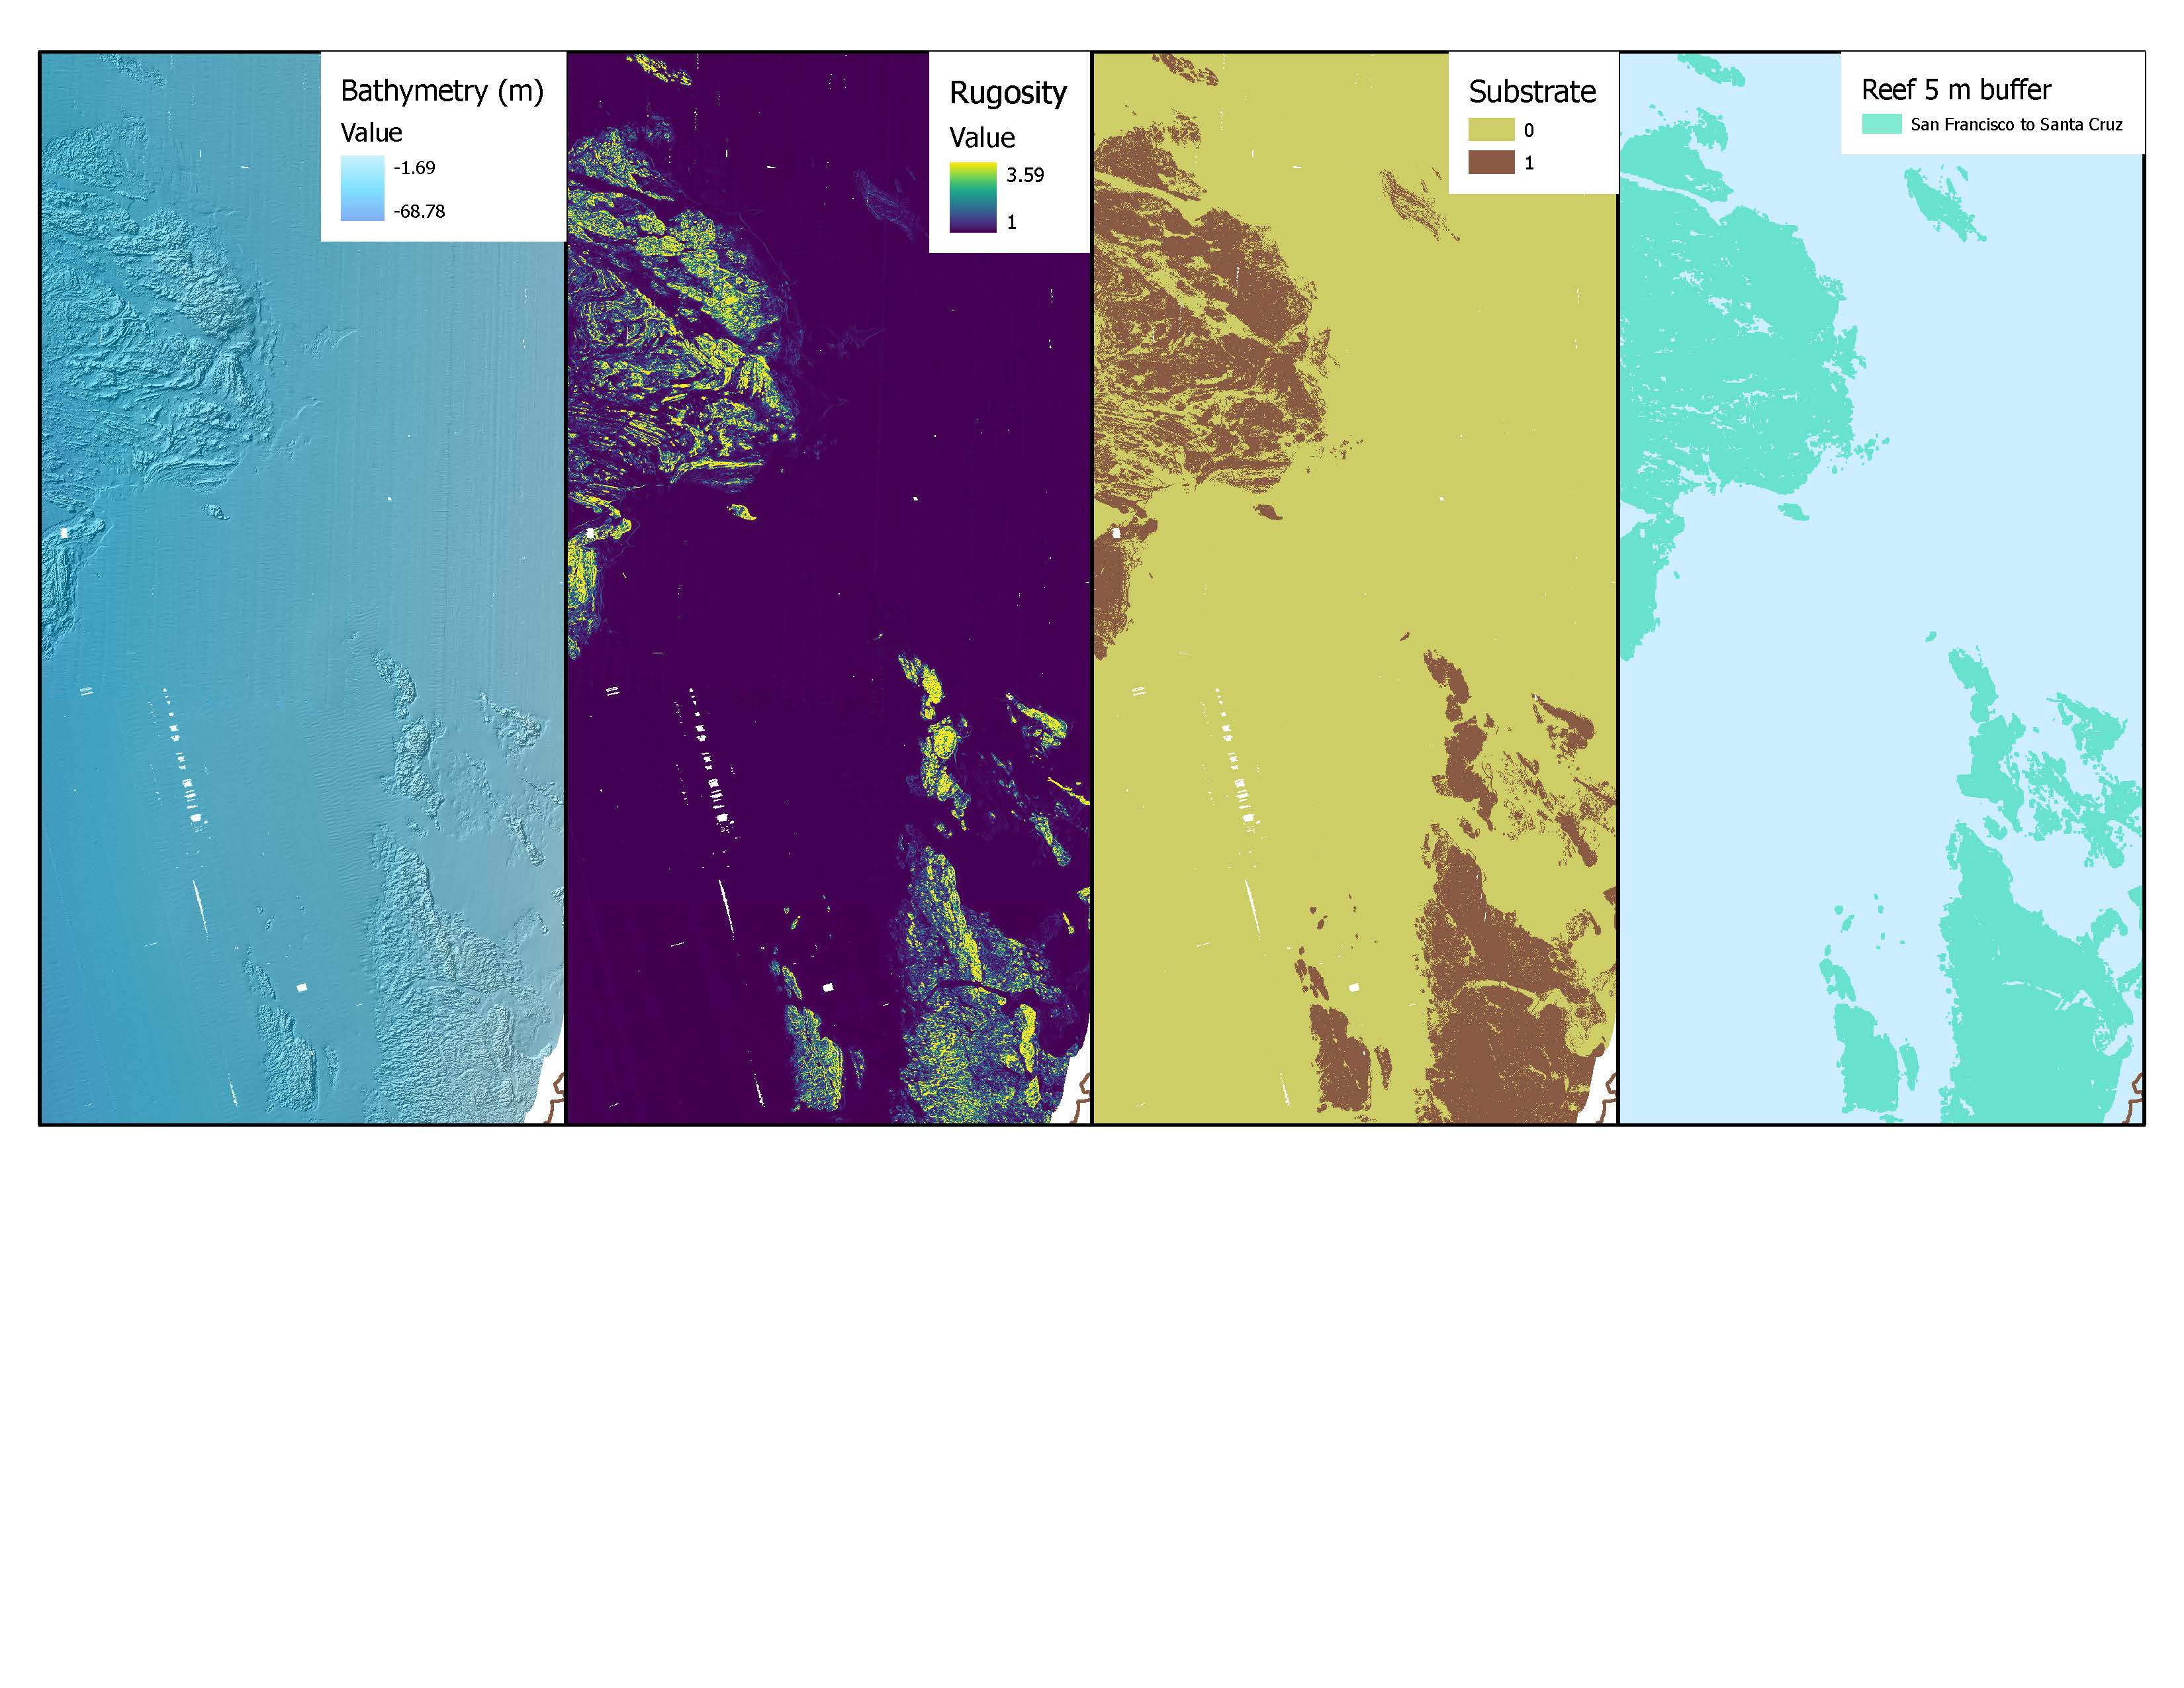
\includegraphics{figures/map_2.jpg}

}

\caption{\label{fig-map2}A example of the high resolution bathymetric
data and components of bathymetry and rugosity used to define rough
versus smooth substrate (where hard substrate is denoted by 1). The far
right panel displays the hard substrate with the added 5 m buffer to
represent the rocky reef habitat.}

\end{figure}

\begin{figure}

{\centering 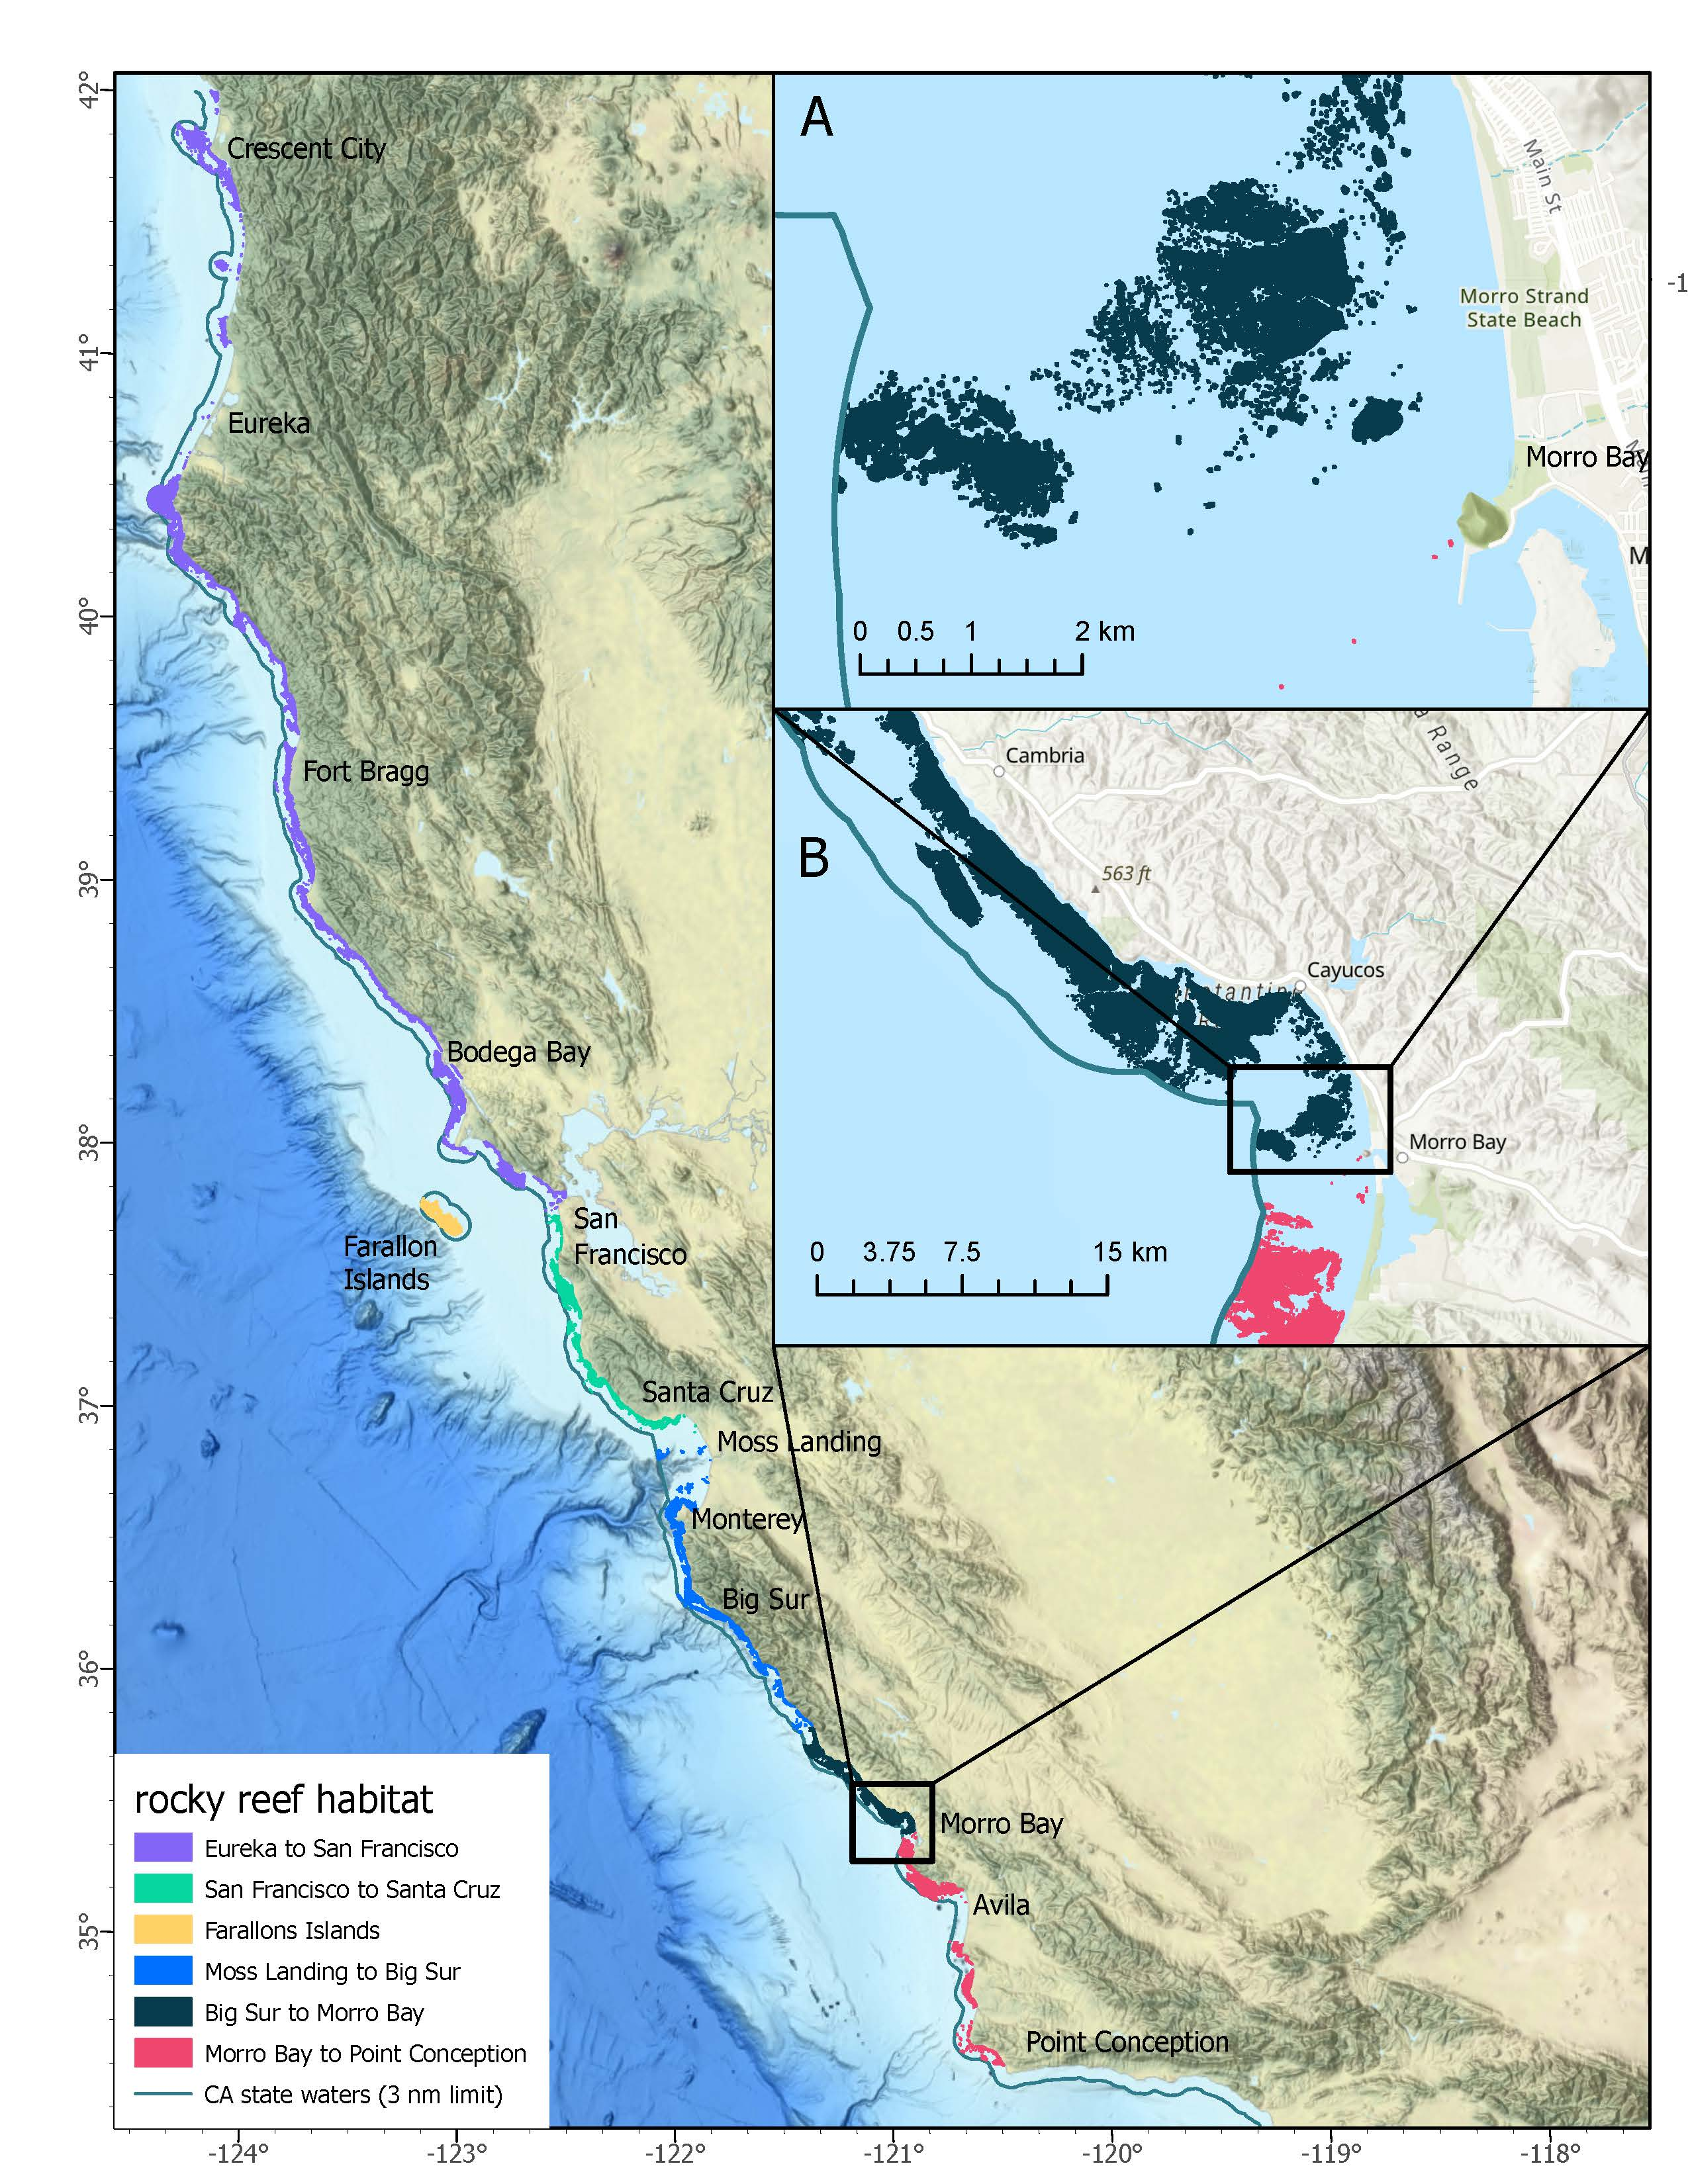
\includegraphics{figures/map.jpg}

}

\caption{\label{fig-map}A maps of California state waters north of Point
Conception colored by the aggregated areas of rocky reef habitat,
including inset A depicting the rocky reef habitat in relation to 3 nm
state water boundary state waters and inset B showing the high
resolution rocky habitat in the area.}

\end{figure}

\begin{figure}

{\centering \includegraphics{figures/percentpositives_map.jpg}

}

\caption{\label{fig-percentpos}The percent of drifts that retained the
target species, within grouped areas of rocky habitat over all years of
the time series. The grey dashed lines represent the aggregated rocky
habitat used to develop an index of abundance.}

\end{figure}

\begin{figure}

{\centering 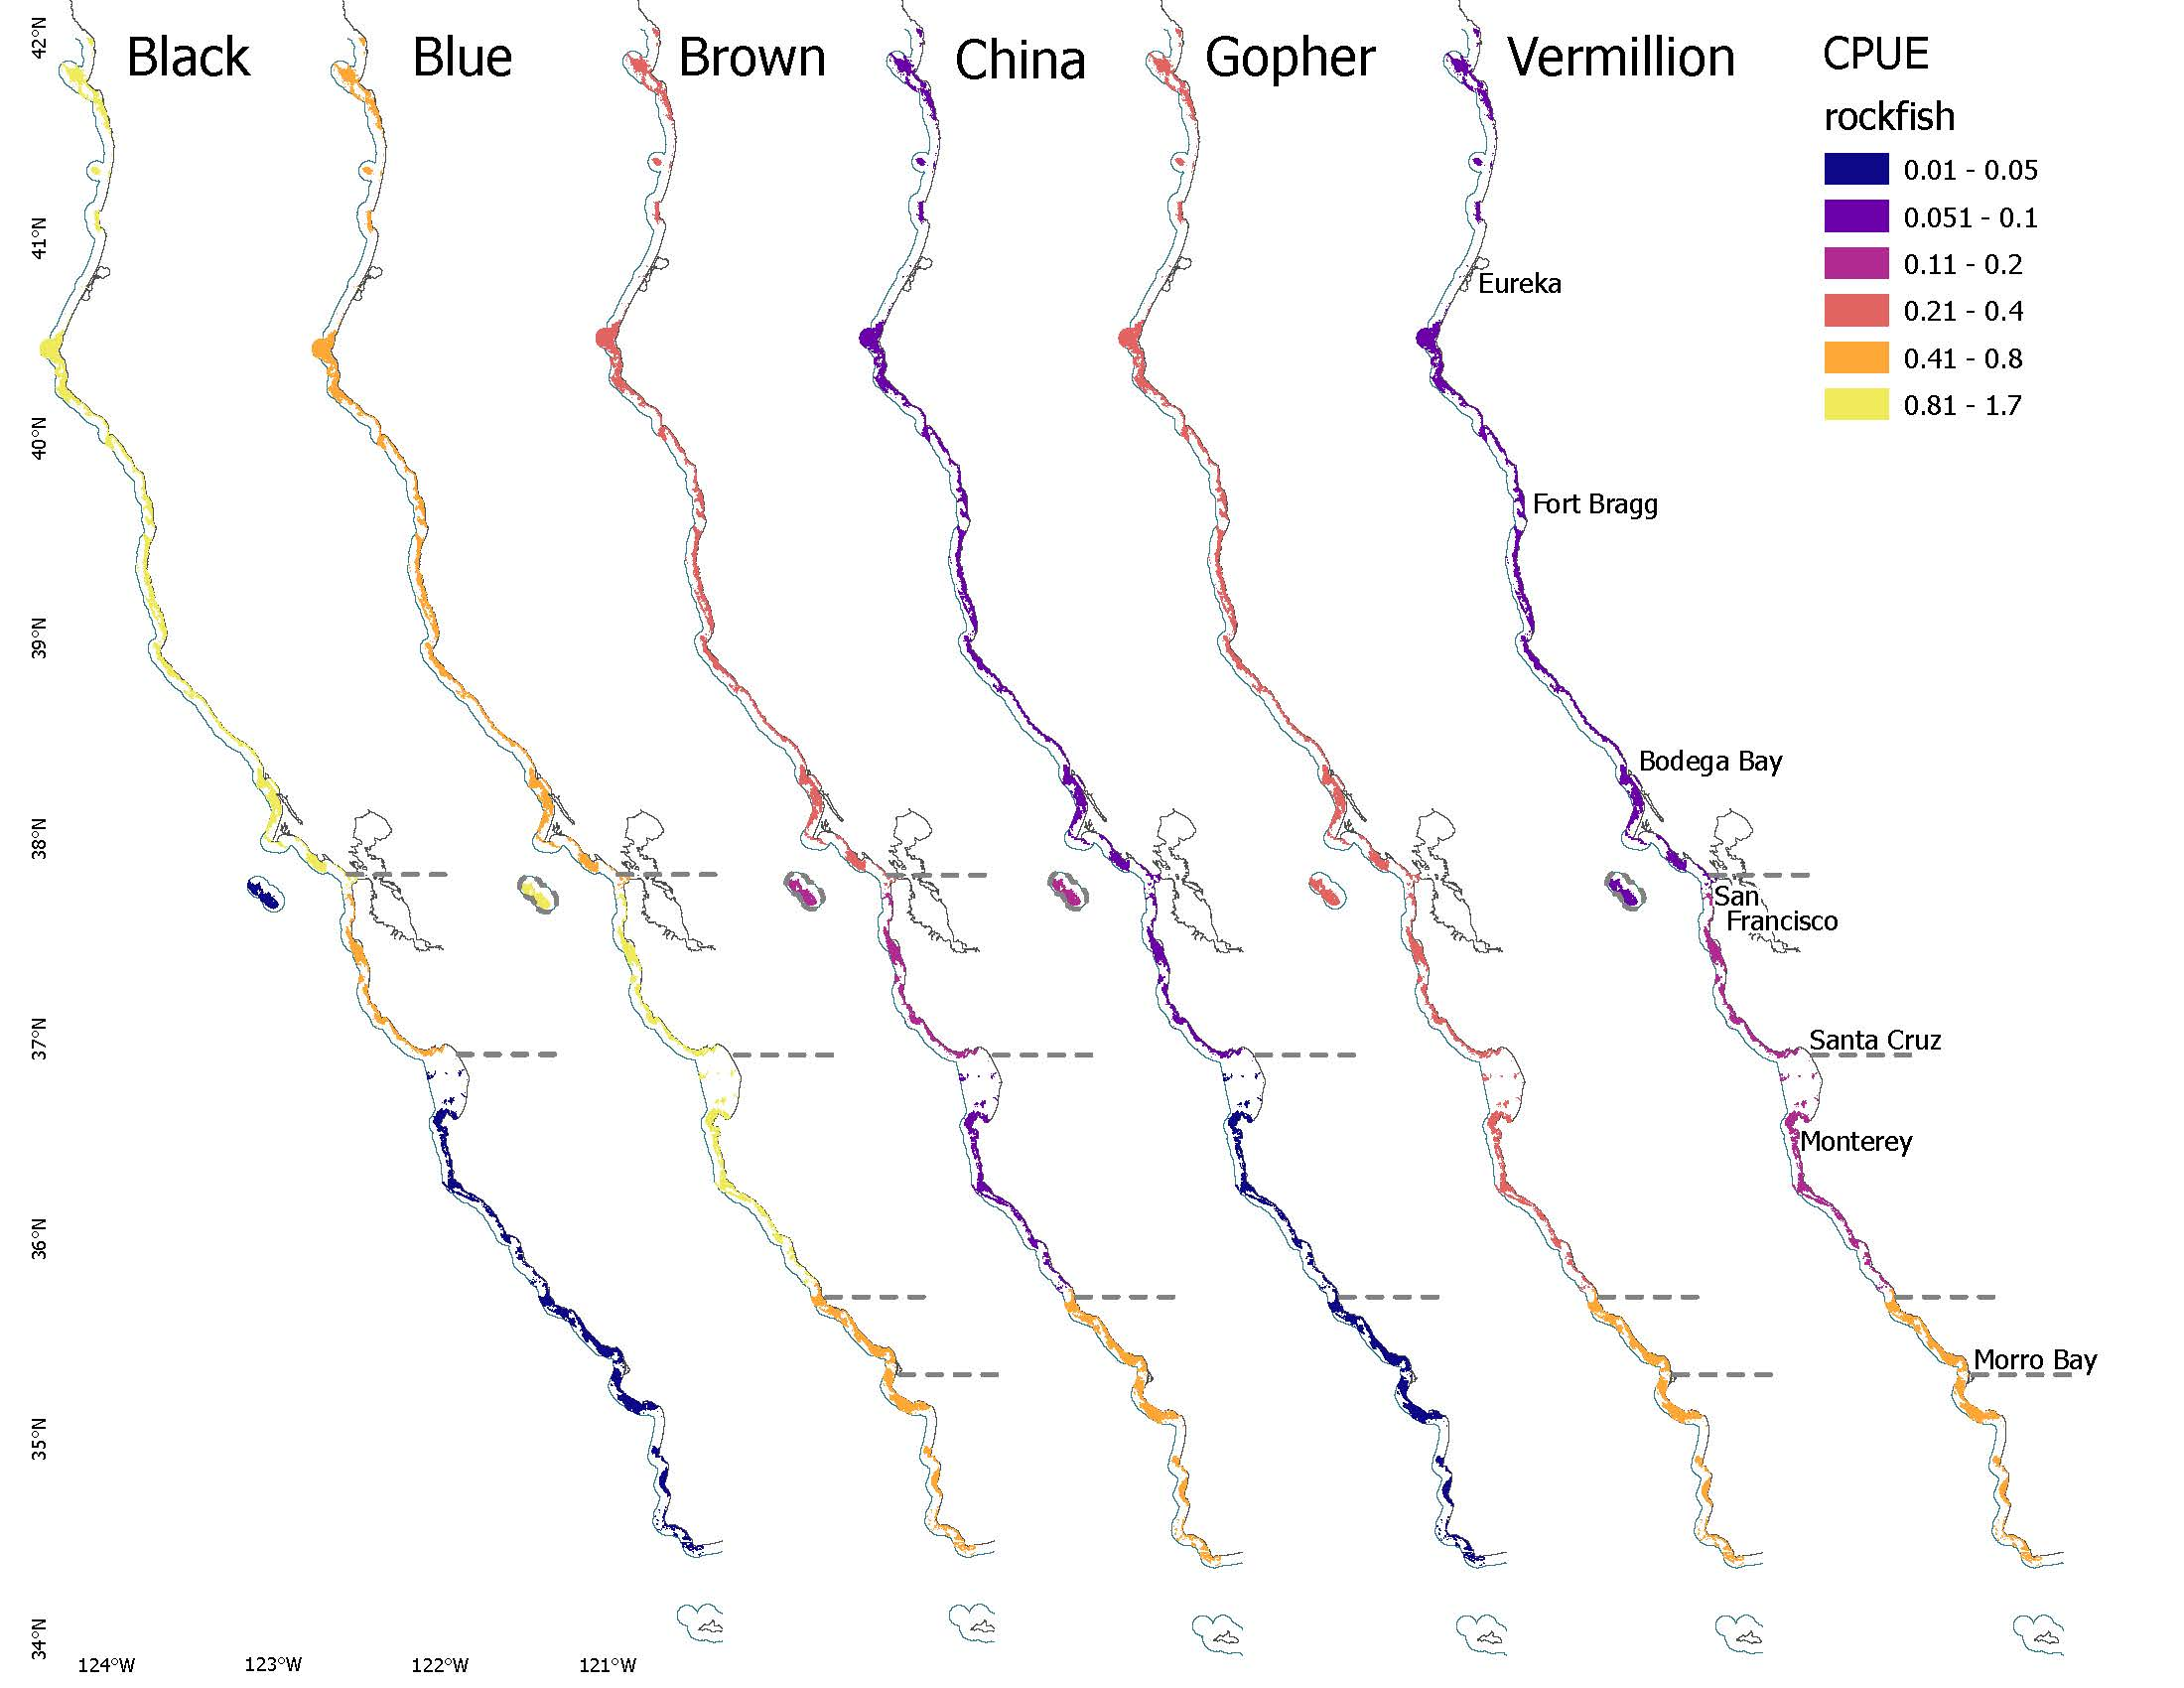
\includegraphics{figures/CPUE_map.jpg}

}

\caption{\label{fig-cpue}The average CPUE across all years of the time
series for each of the six species. The grey dashed lines represent the
aggregated rocky habitat used to develop an index of abundance.}

\end{figure}

\begin{figure}

\begin{minipage}[t]{0.50\linewidth}

{\centering 

\raisebox{-\height}{

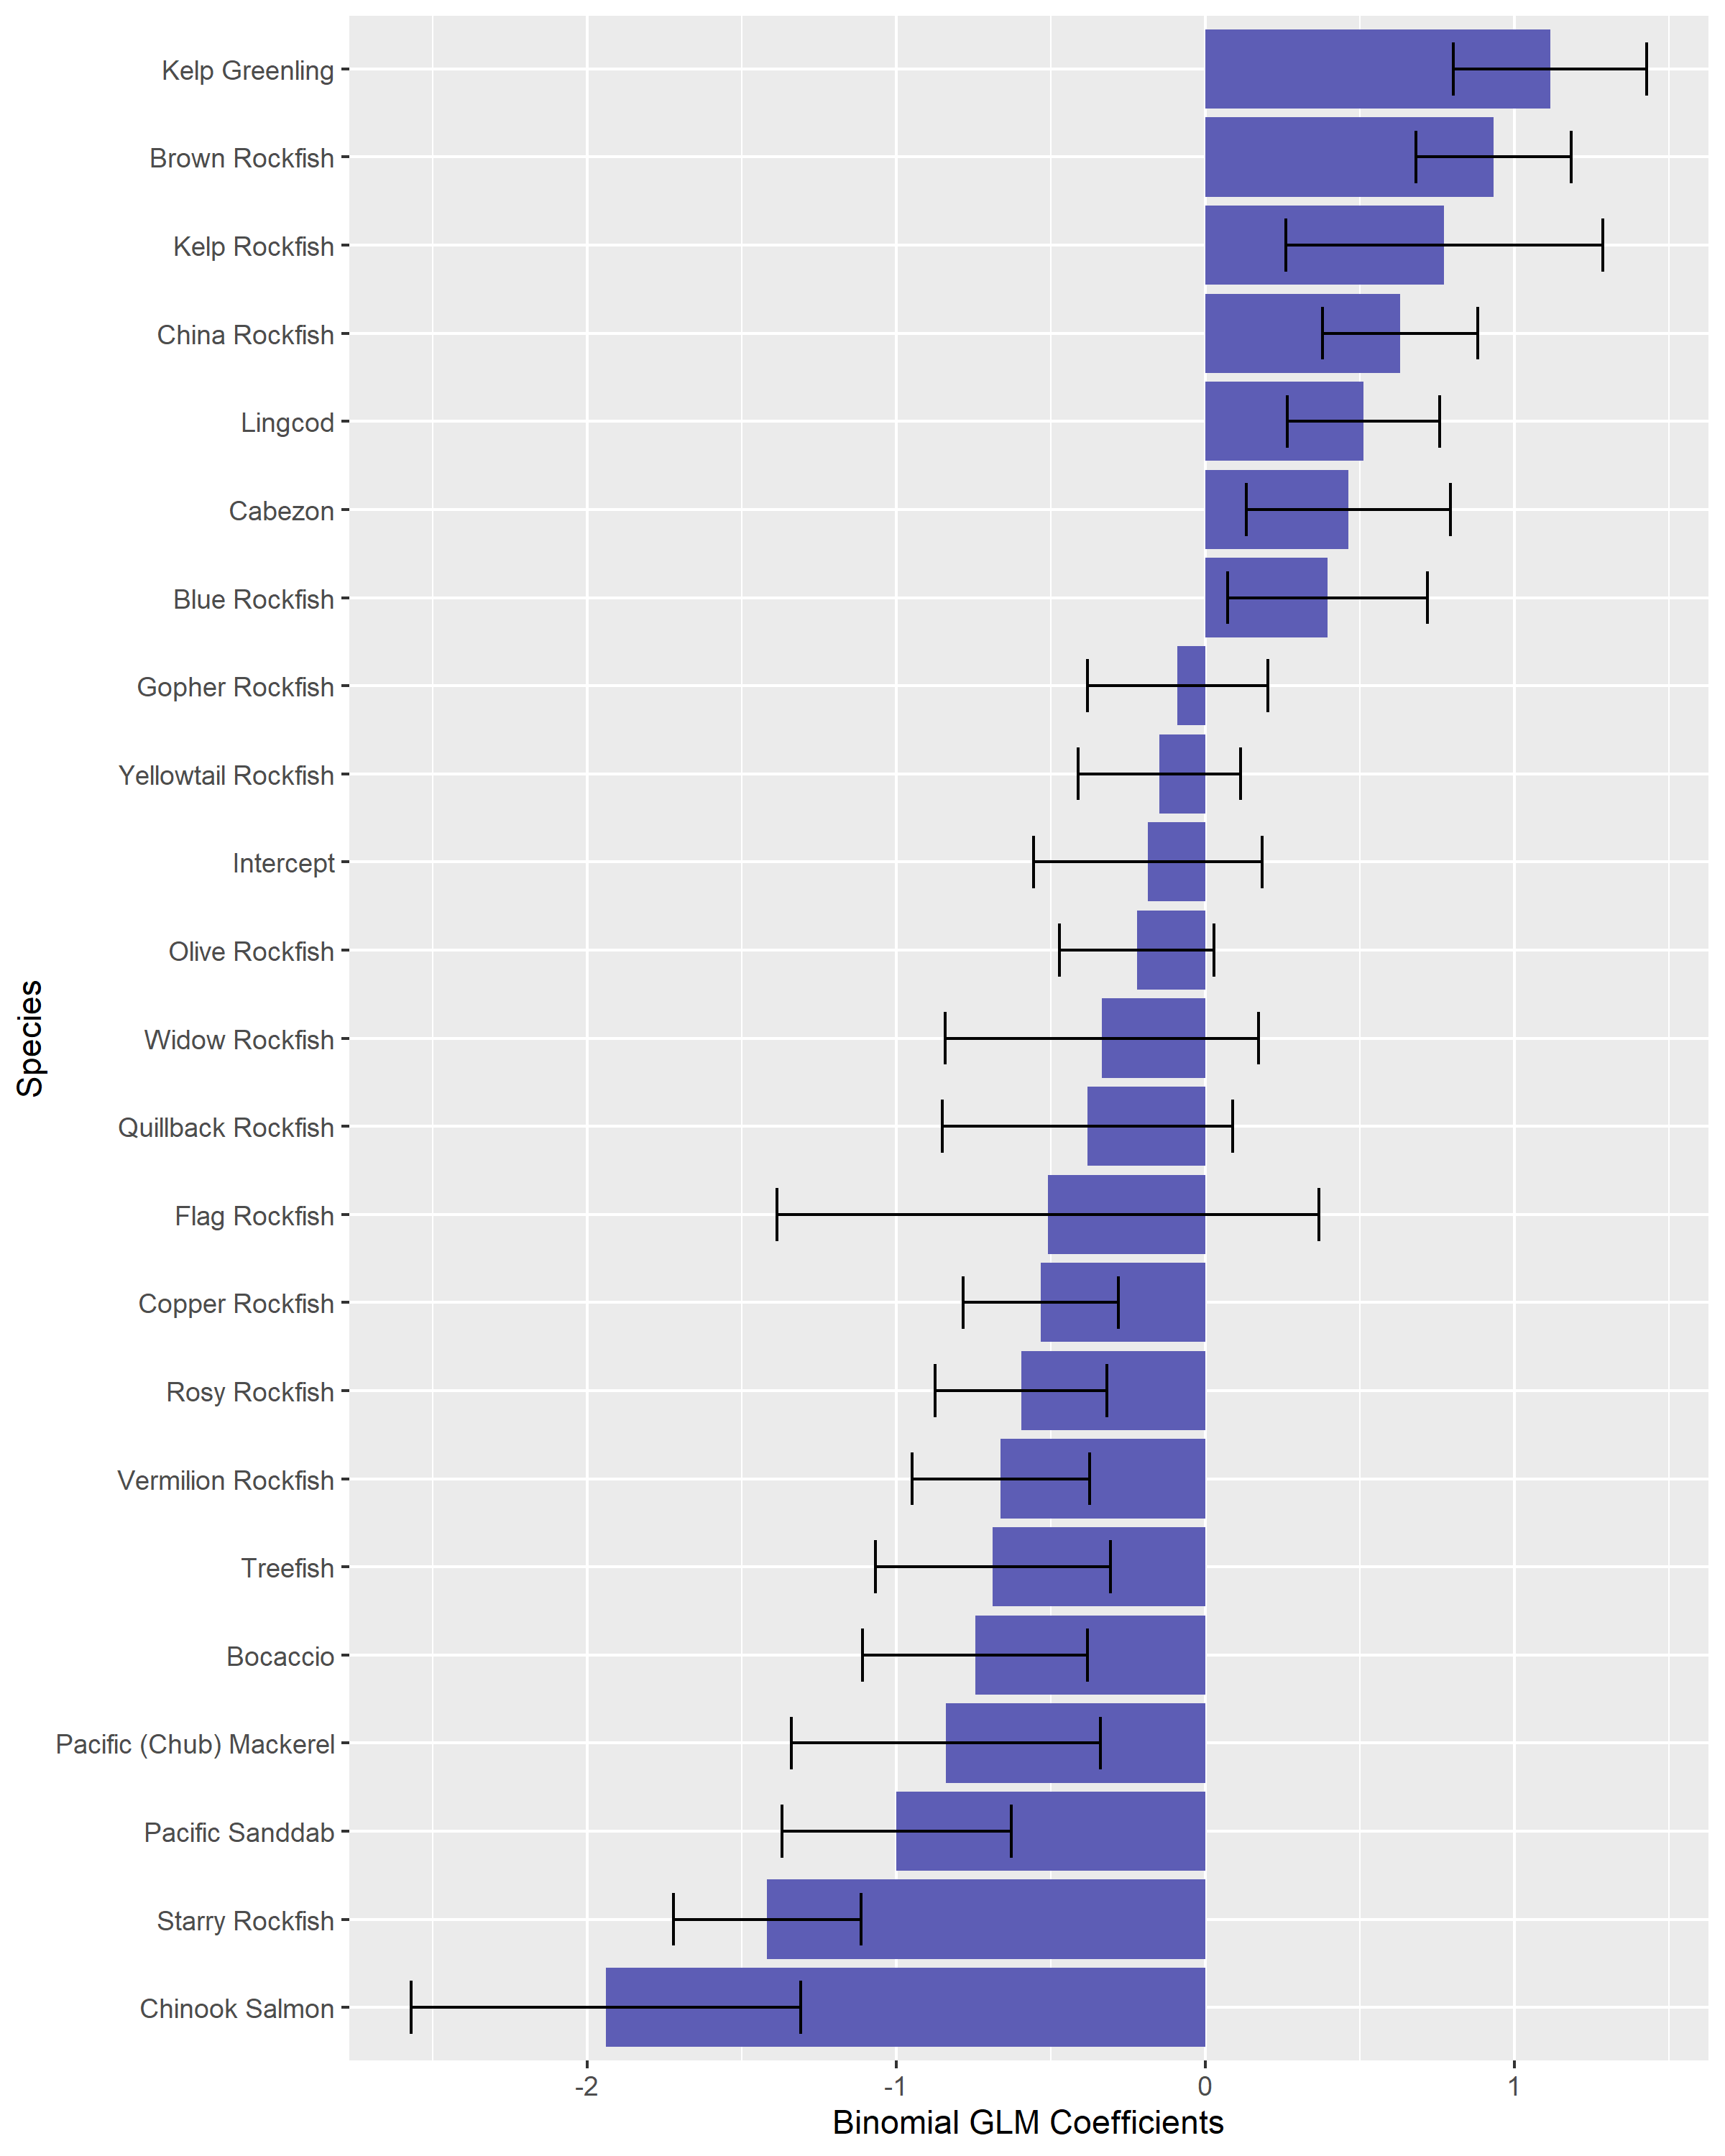
\includegraphics[width=2.7in,height=\textheight]{figures/black_trip_sm.png}

}

}

\subcaption{\label{fig-black-tripsm}Black rockfish trip-level}
\end{minipage}%
%
\begin{minipage}[t]{0.50\linewidth}

{\centering 

\raisebox{-\height}{

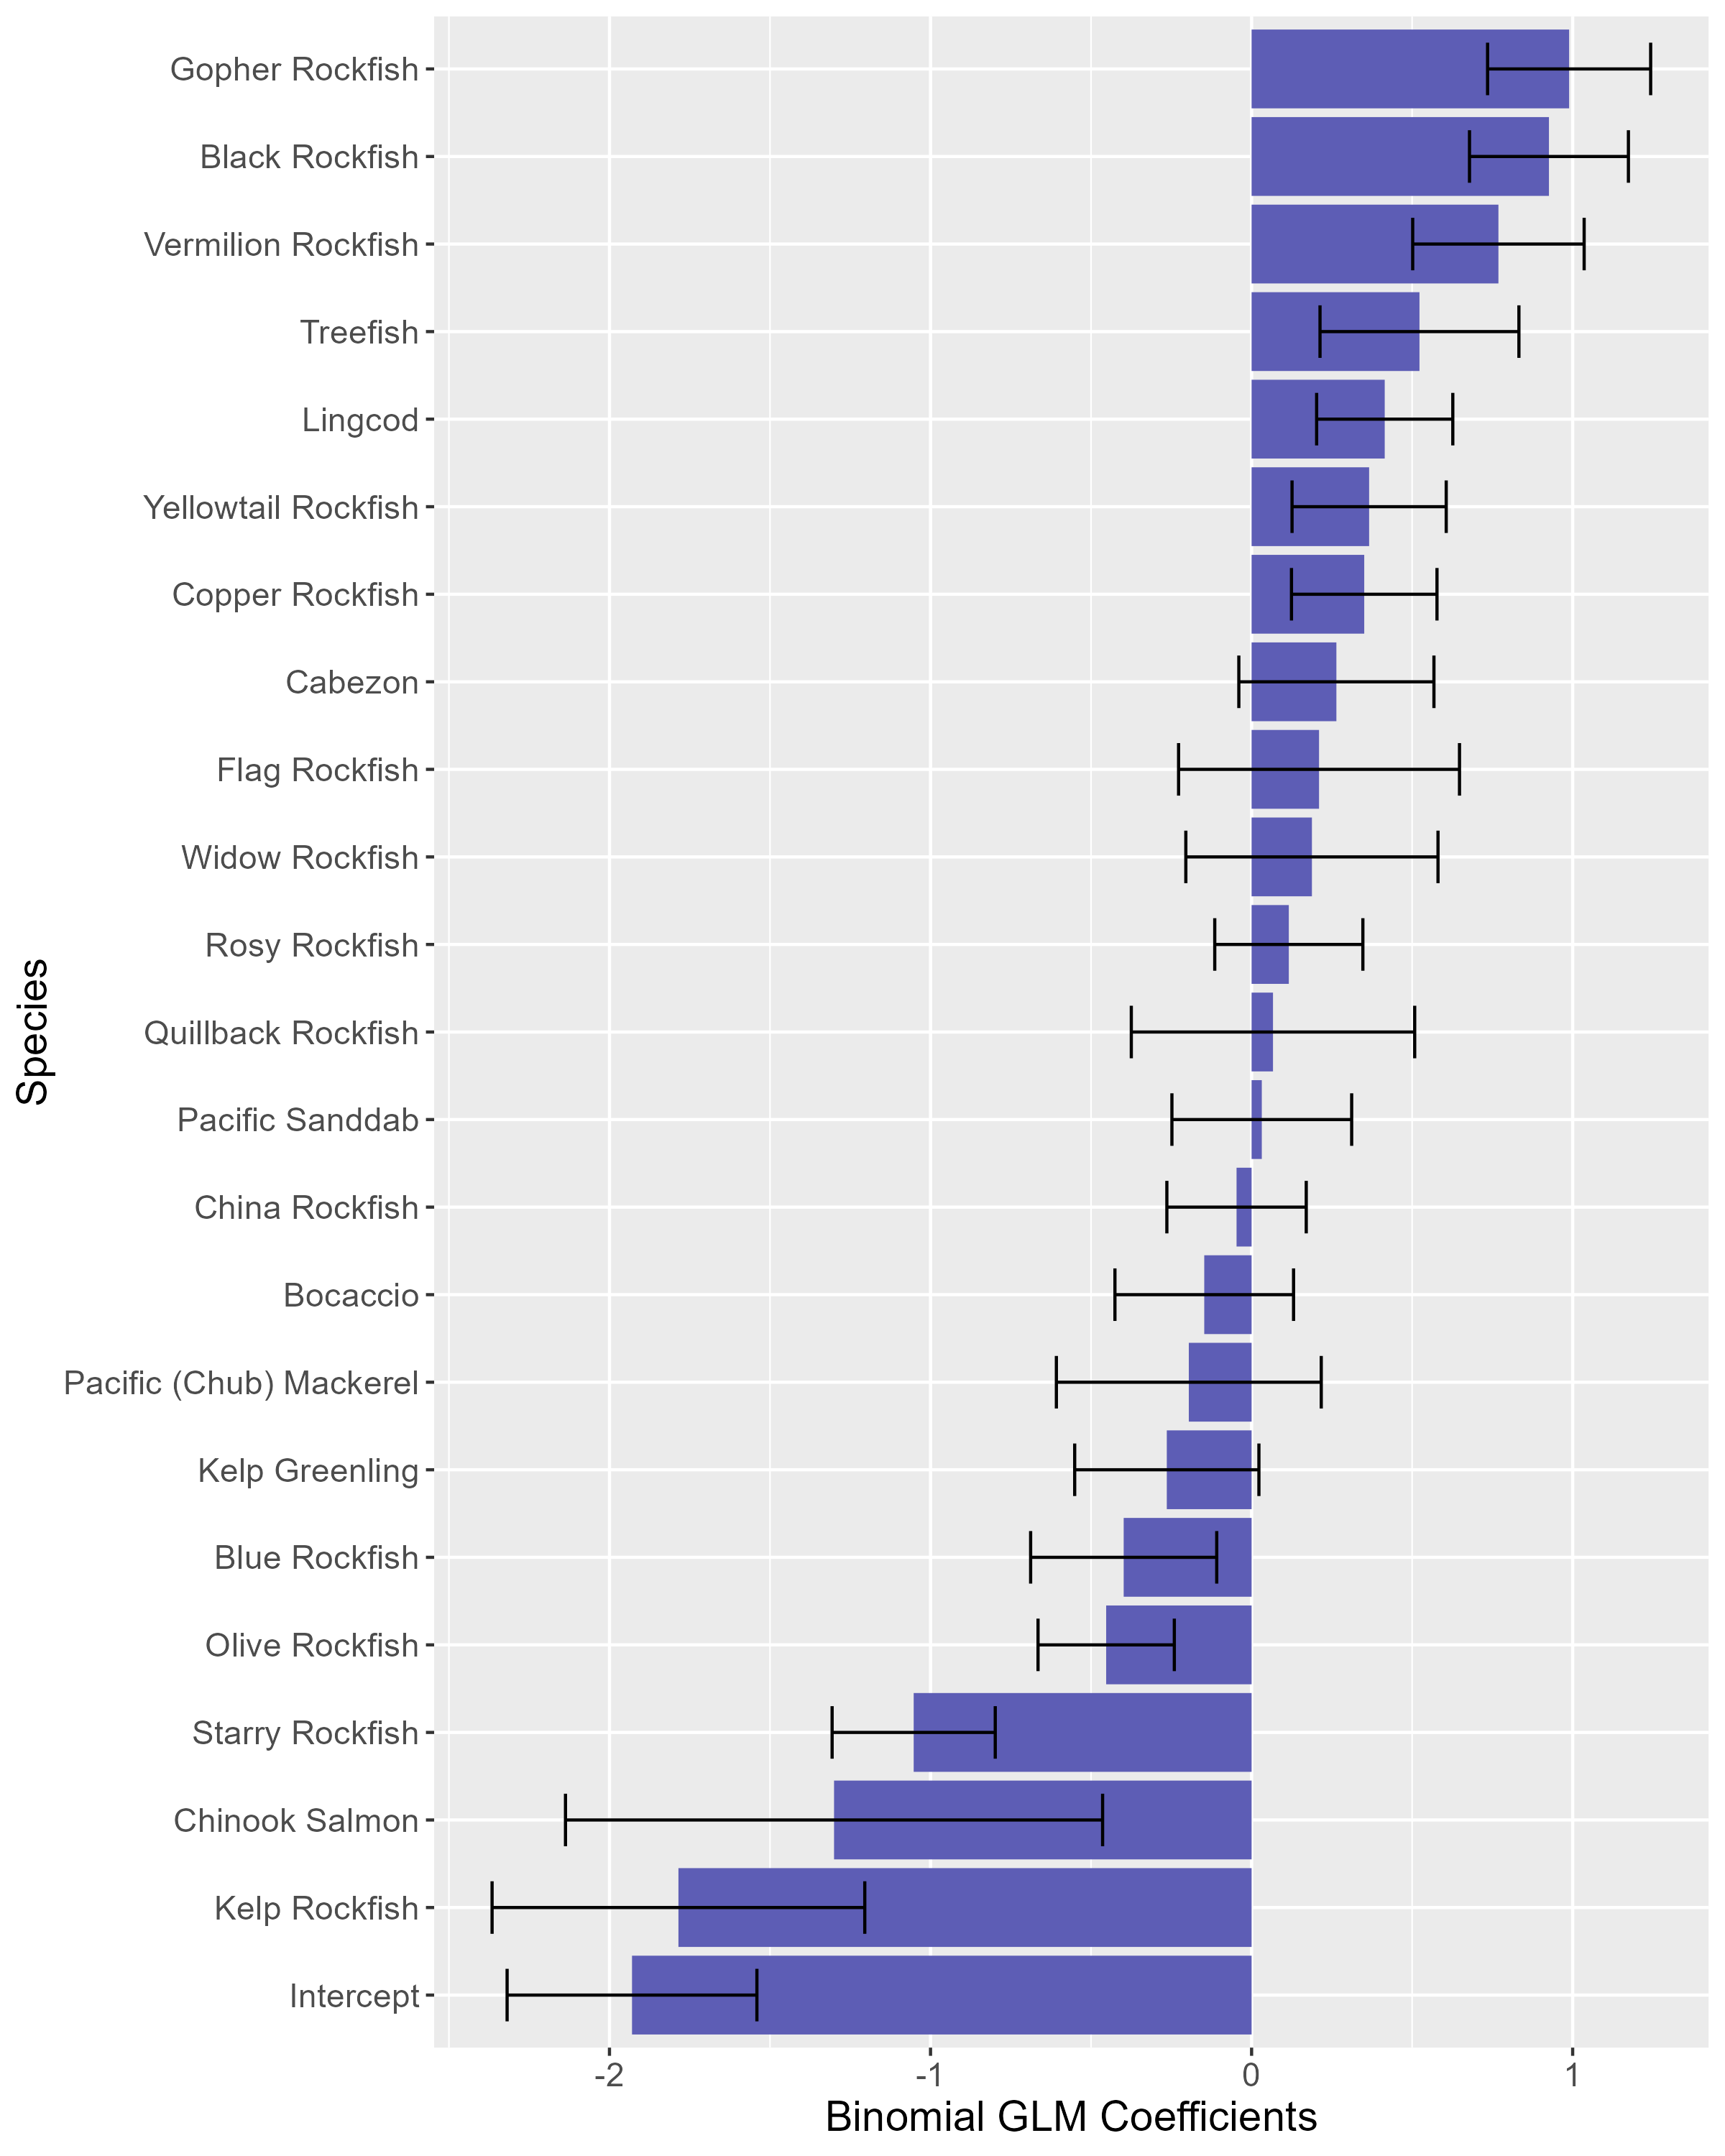
\includegraphics[width=2.7in,height=\textheight]{figures/brown_trip_sm.png}

}

}

\subcaption{\label{fig-brown-tripsm}Brown rockfish trip-level}
\end{minipage}%

\caption{\label{fig-sm}Examples of the species coefficients and 95\%
confidence intervals for the Stephens-MacCall filtering for black
rockfish (a) and brown rockfish (b) in the trip-level data. A positive
coefficient indicates a species is associated with the target species
and a negative coefficient indicates the species is not associated with
the target species.}

\end{figure}

\begin{figure}

\begin{minipage}[t]{0.50\linewidth}

{\centering 

\raisebox{-\height}{

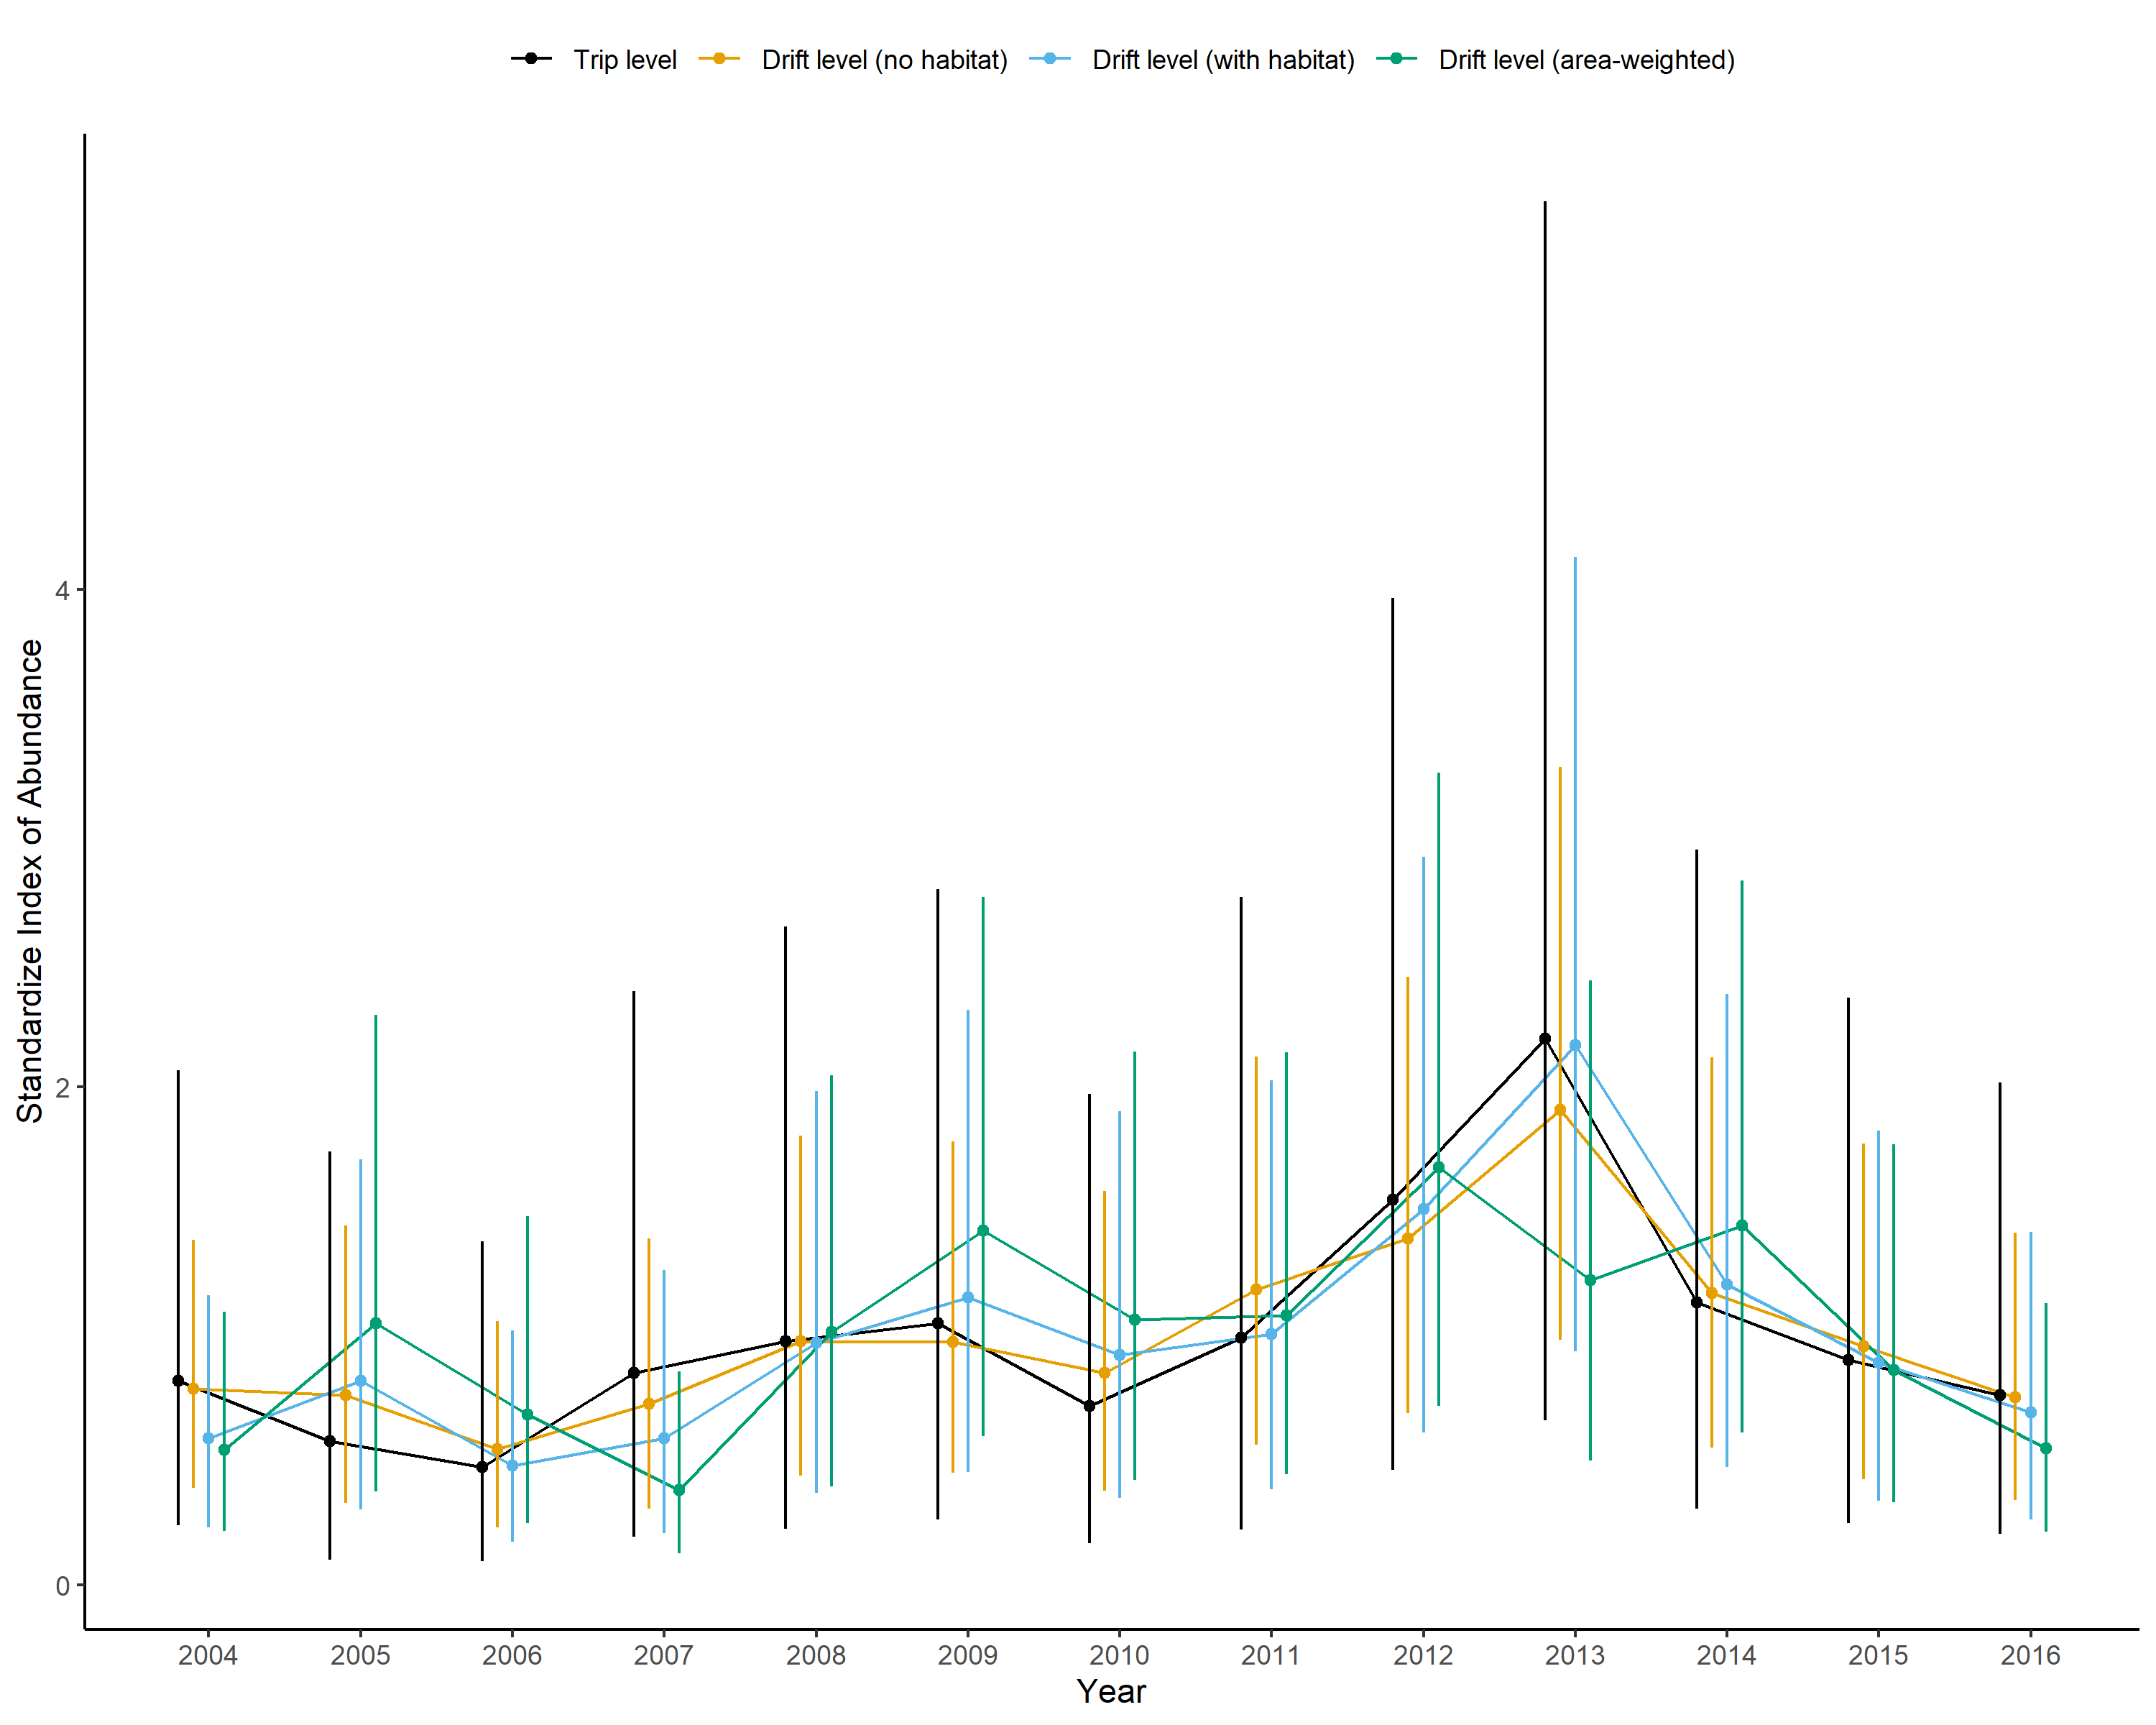
\includegraphics[width=3in,height=\textheight]{figures/black_indices.png}

}

}

\subcaption{\label{fig-black-indices}Black rockfish}
\end{minipage}%
%
\begin{minipage}[t]{0.50\linewidth}

{\centering 

\raisebox{-\height}{

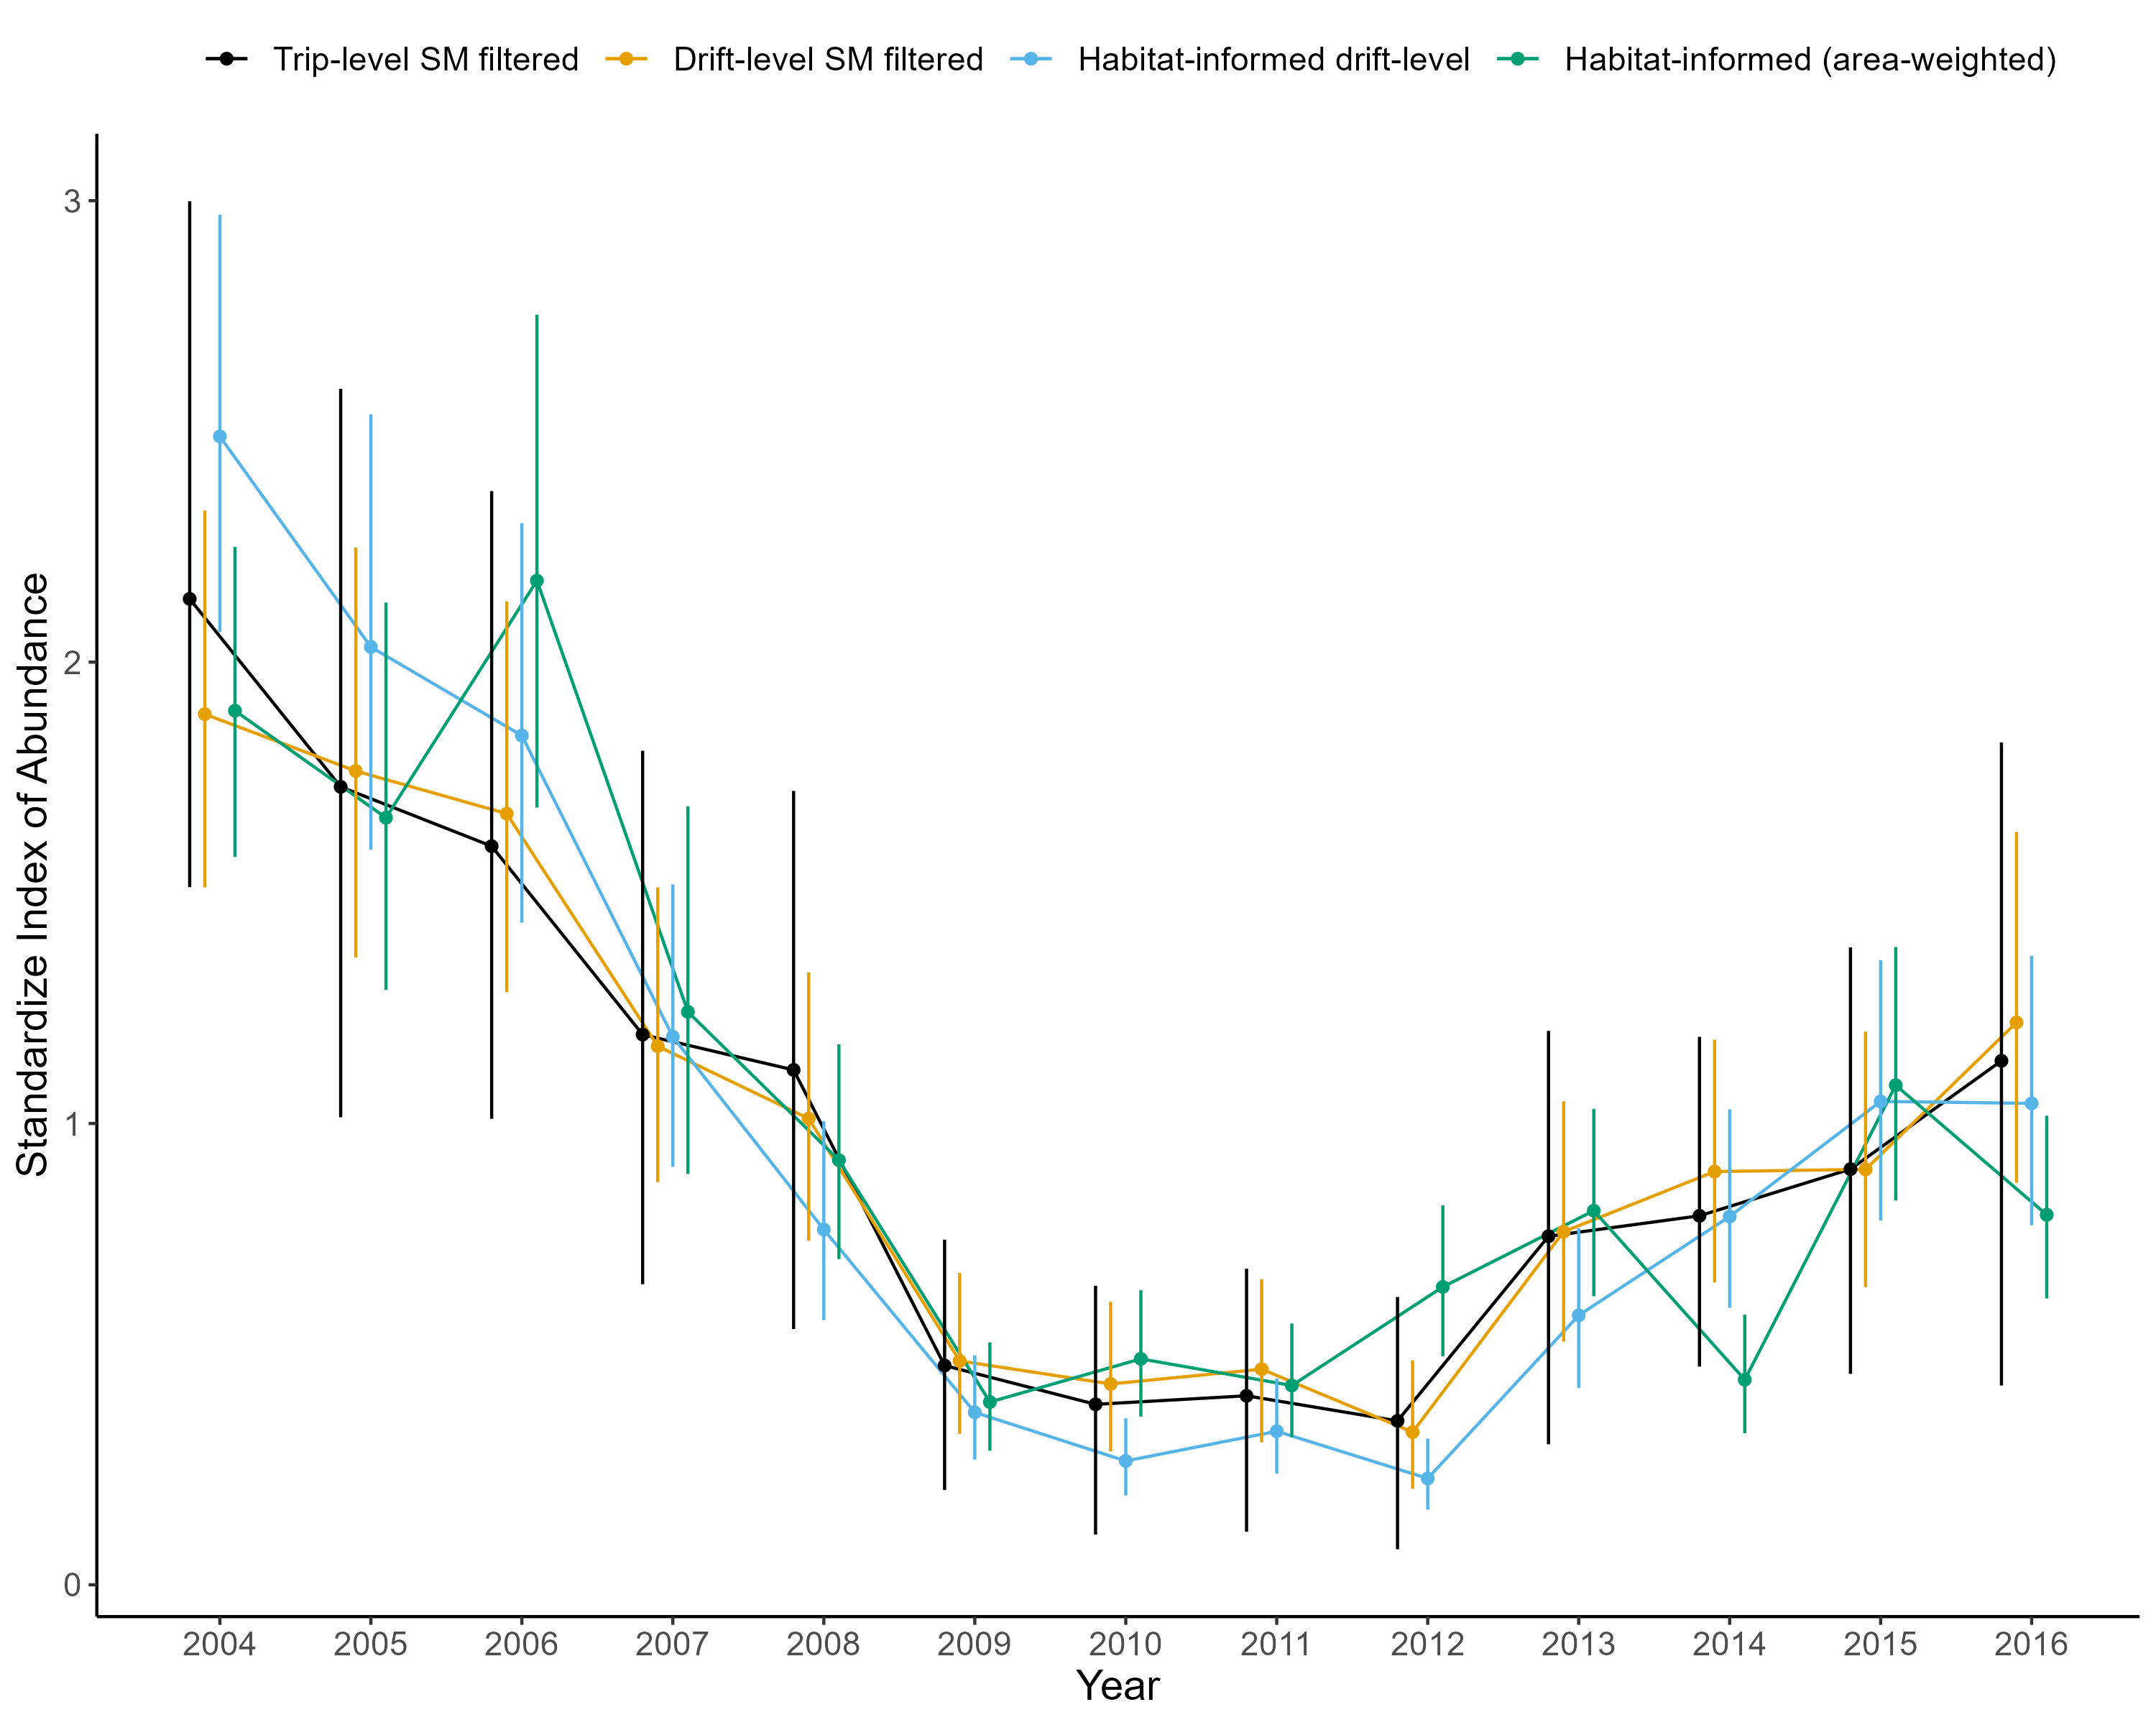
\includegraphics[width=3in,height=\textheight]{figures/blue_indices.png}

}

}

\subcaption{\label{fig-blue-indices}Blue rockfish}
\end{minipage}%
\newline
\begin{minipage}[t]{0.50\linewidth}

{\centering 

\raisebox{-\height}{

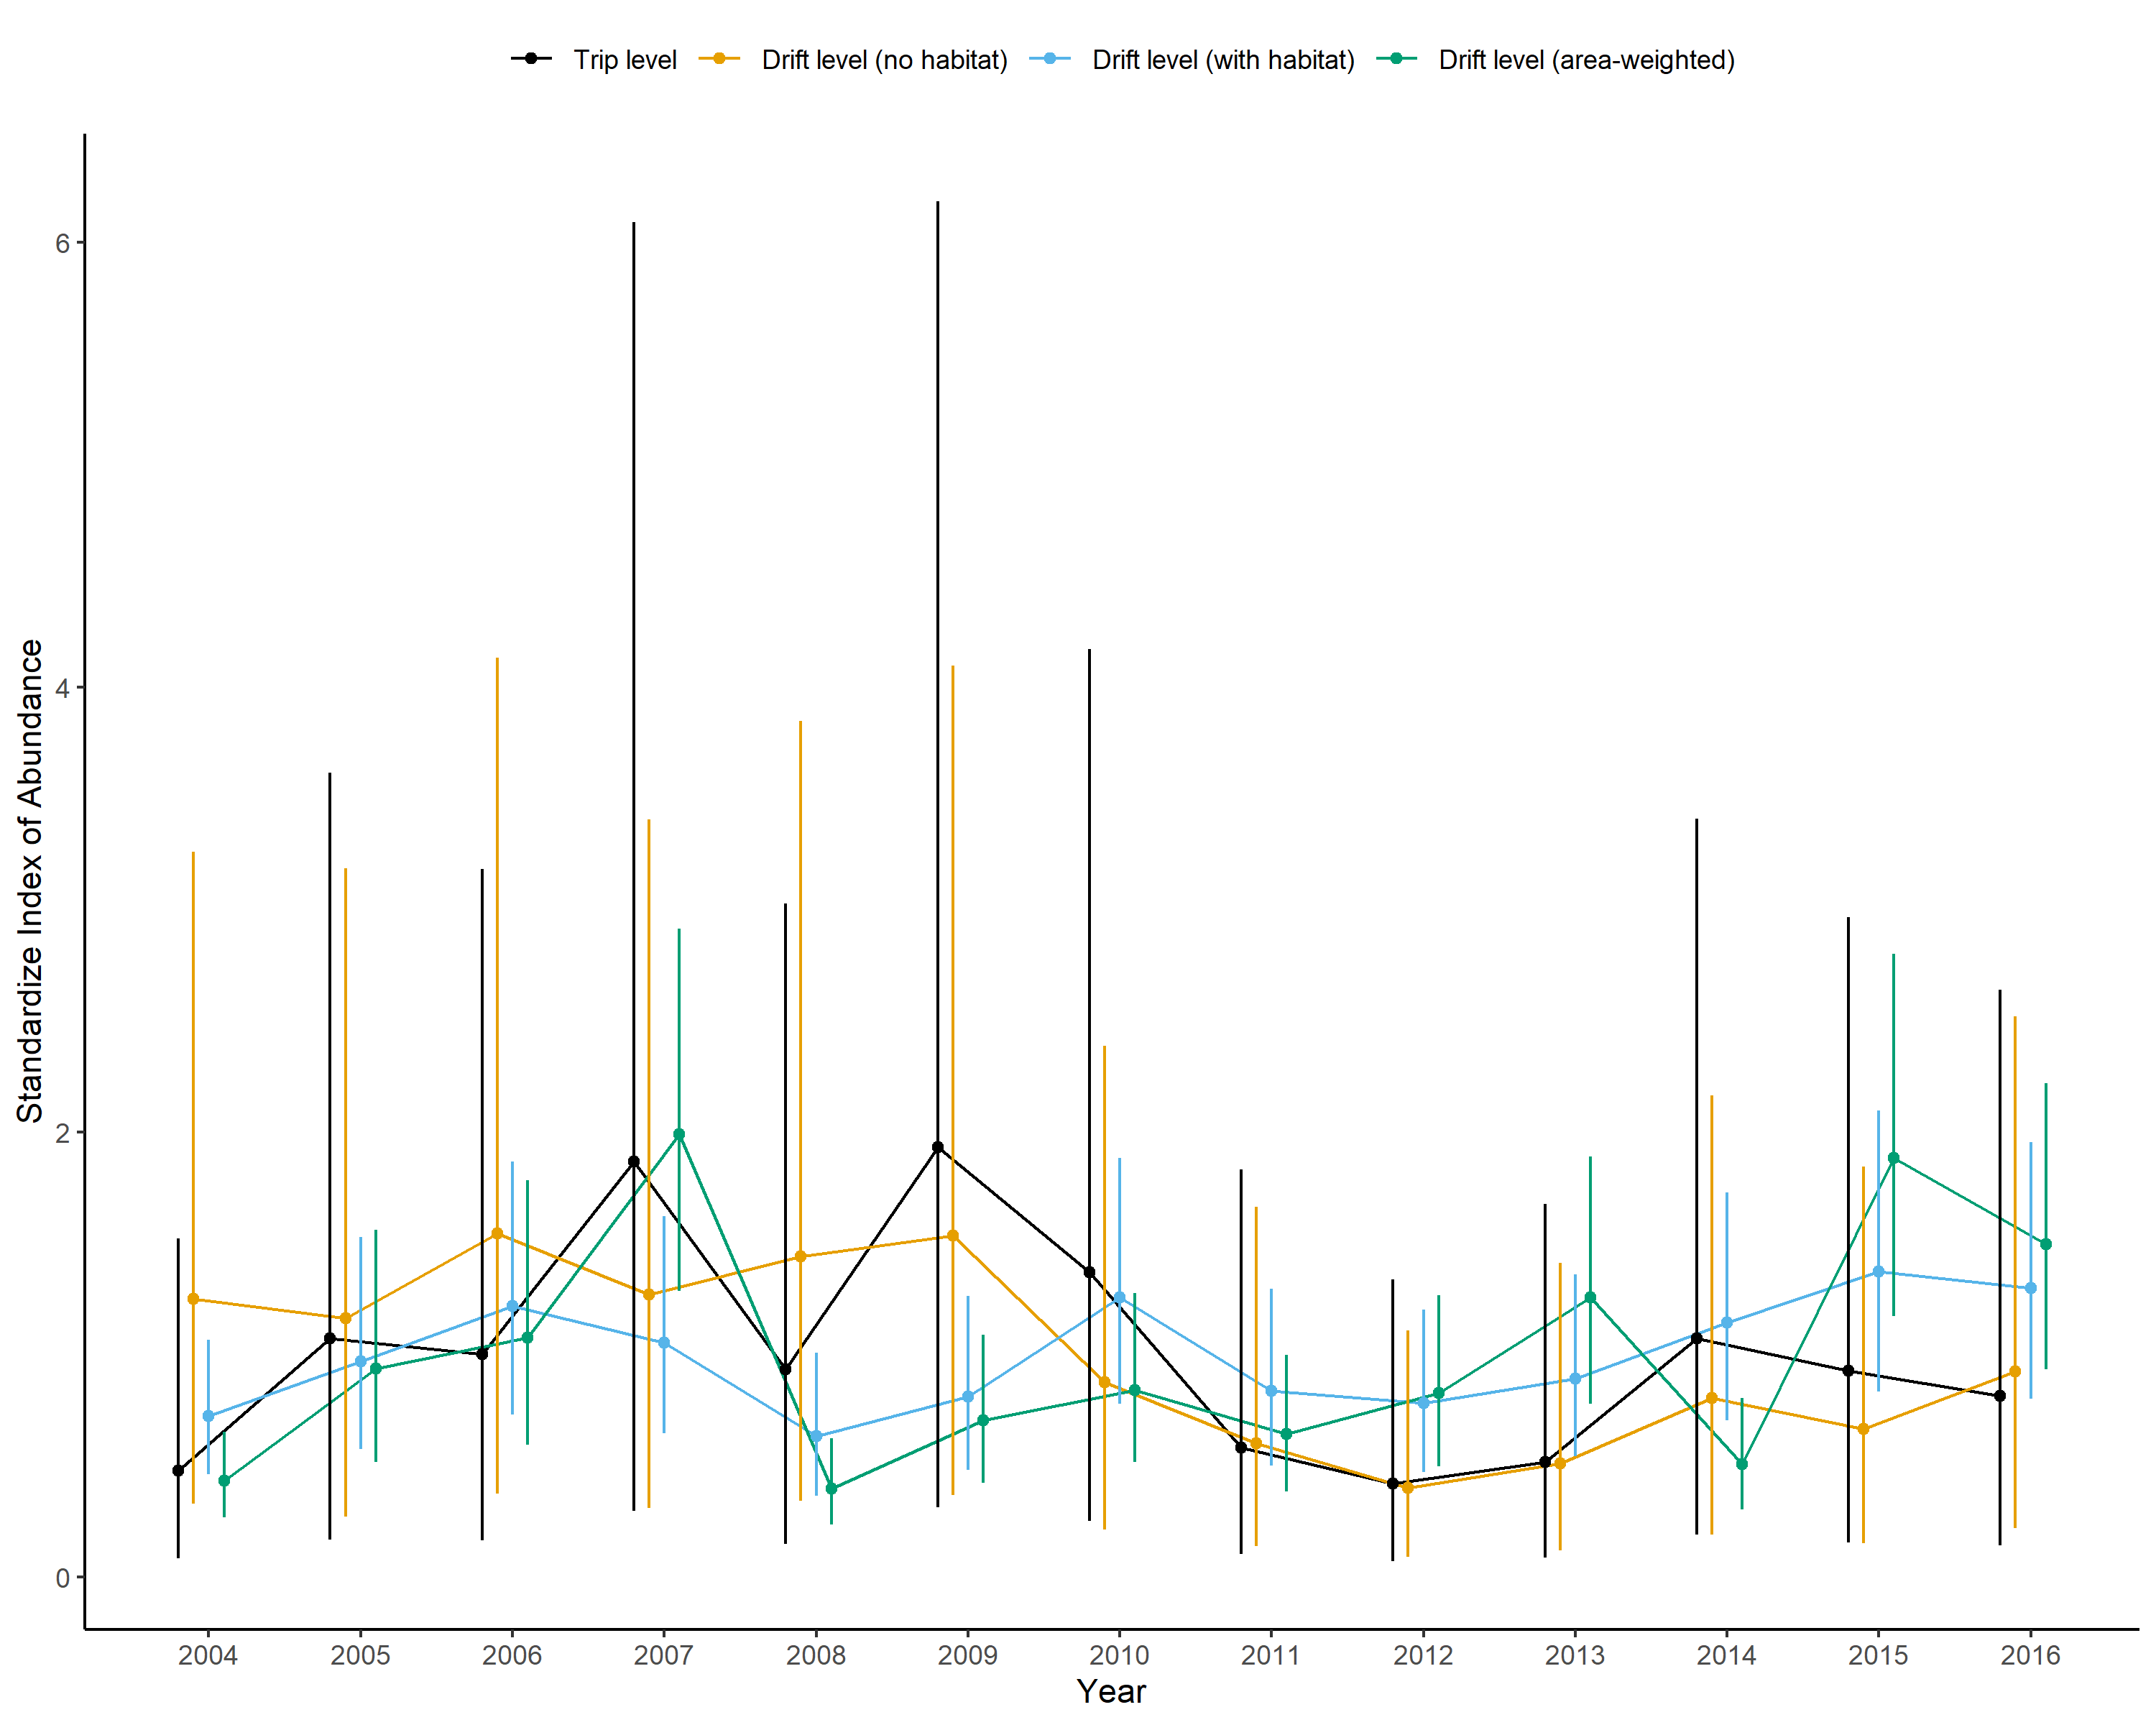
\includegraphics[width=3in,height=\textheight]{figures/brown_indices.png}

}

}

\subcaption{\label{fig-brown-indices}Brown rockfish}
\end{minipage}%
%
\begin{minipage}[t]{0.50\linewidth}

{\centering 

\raisebox{-\height}{

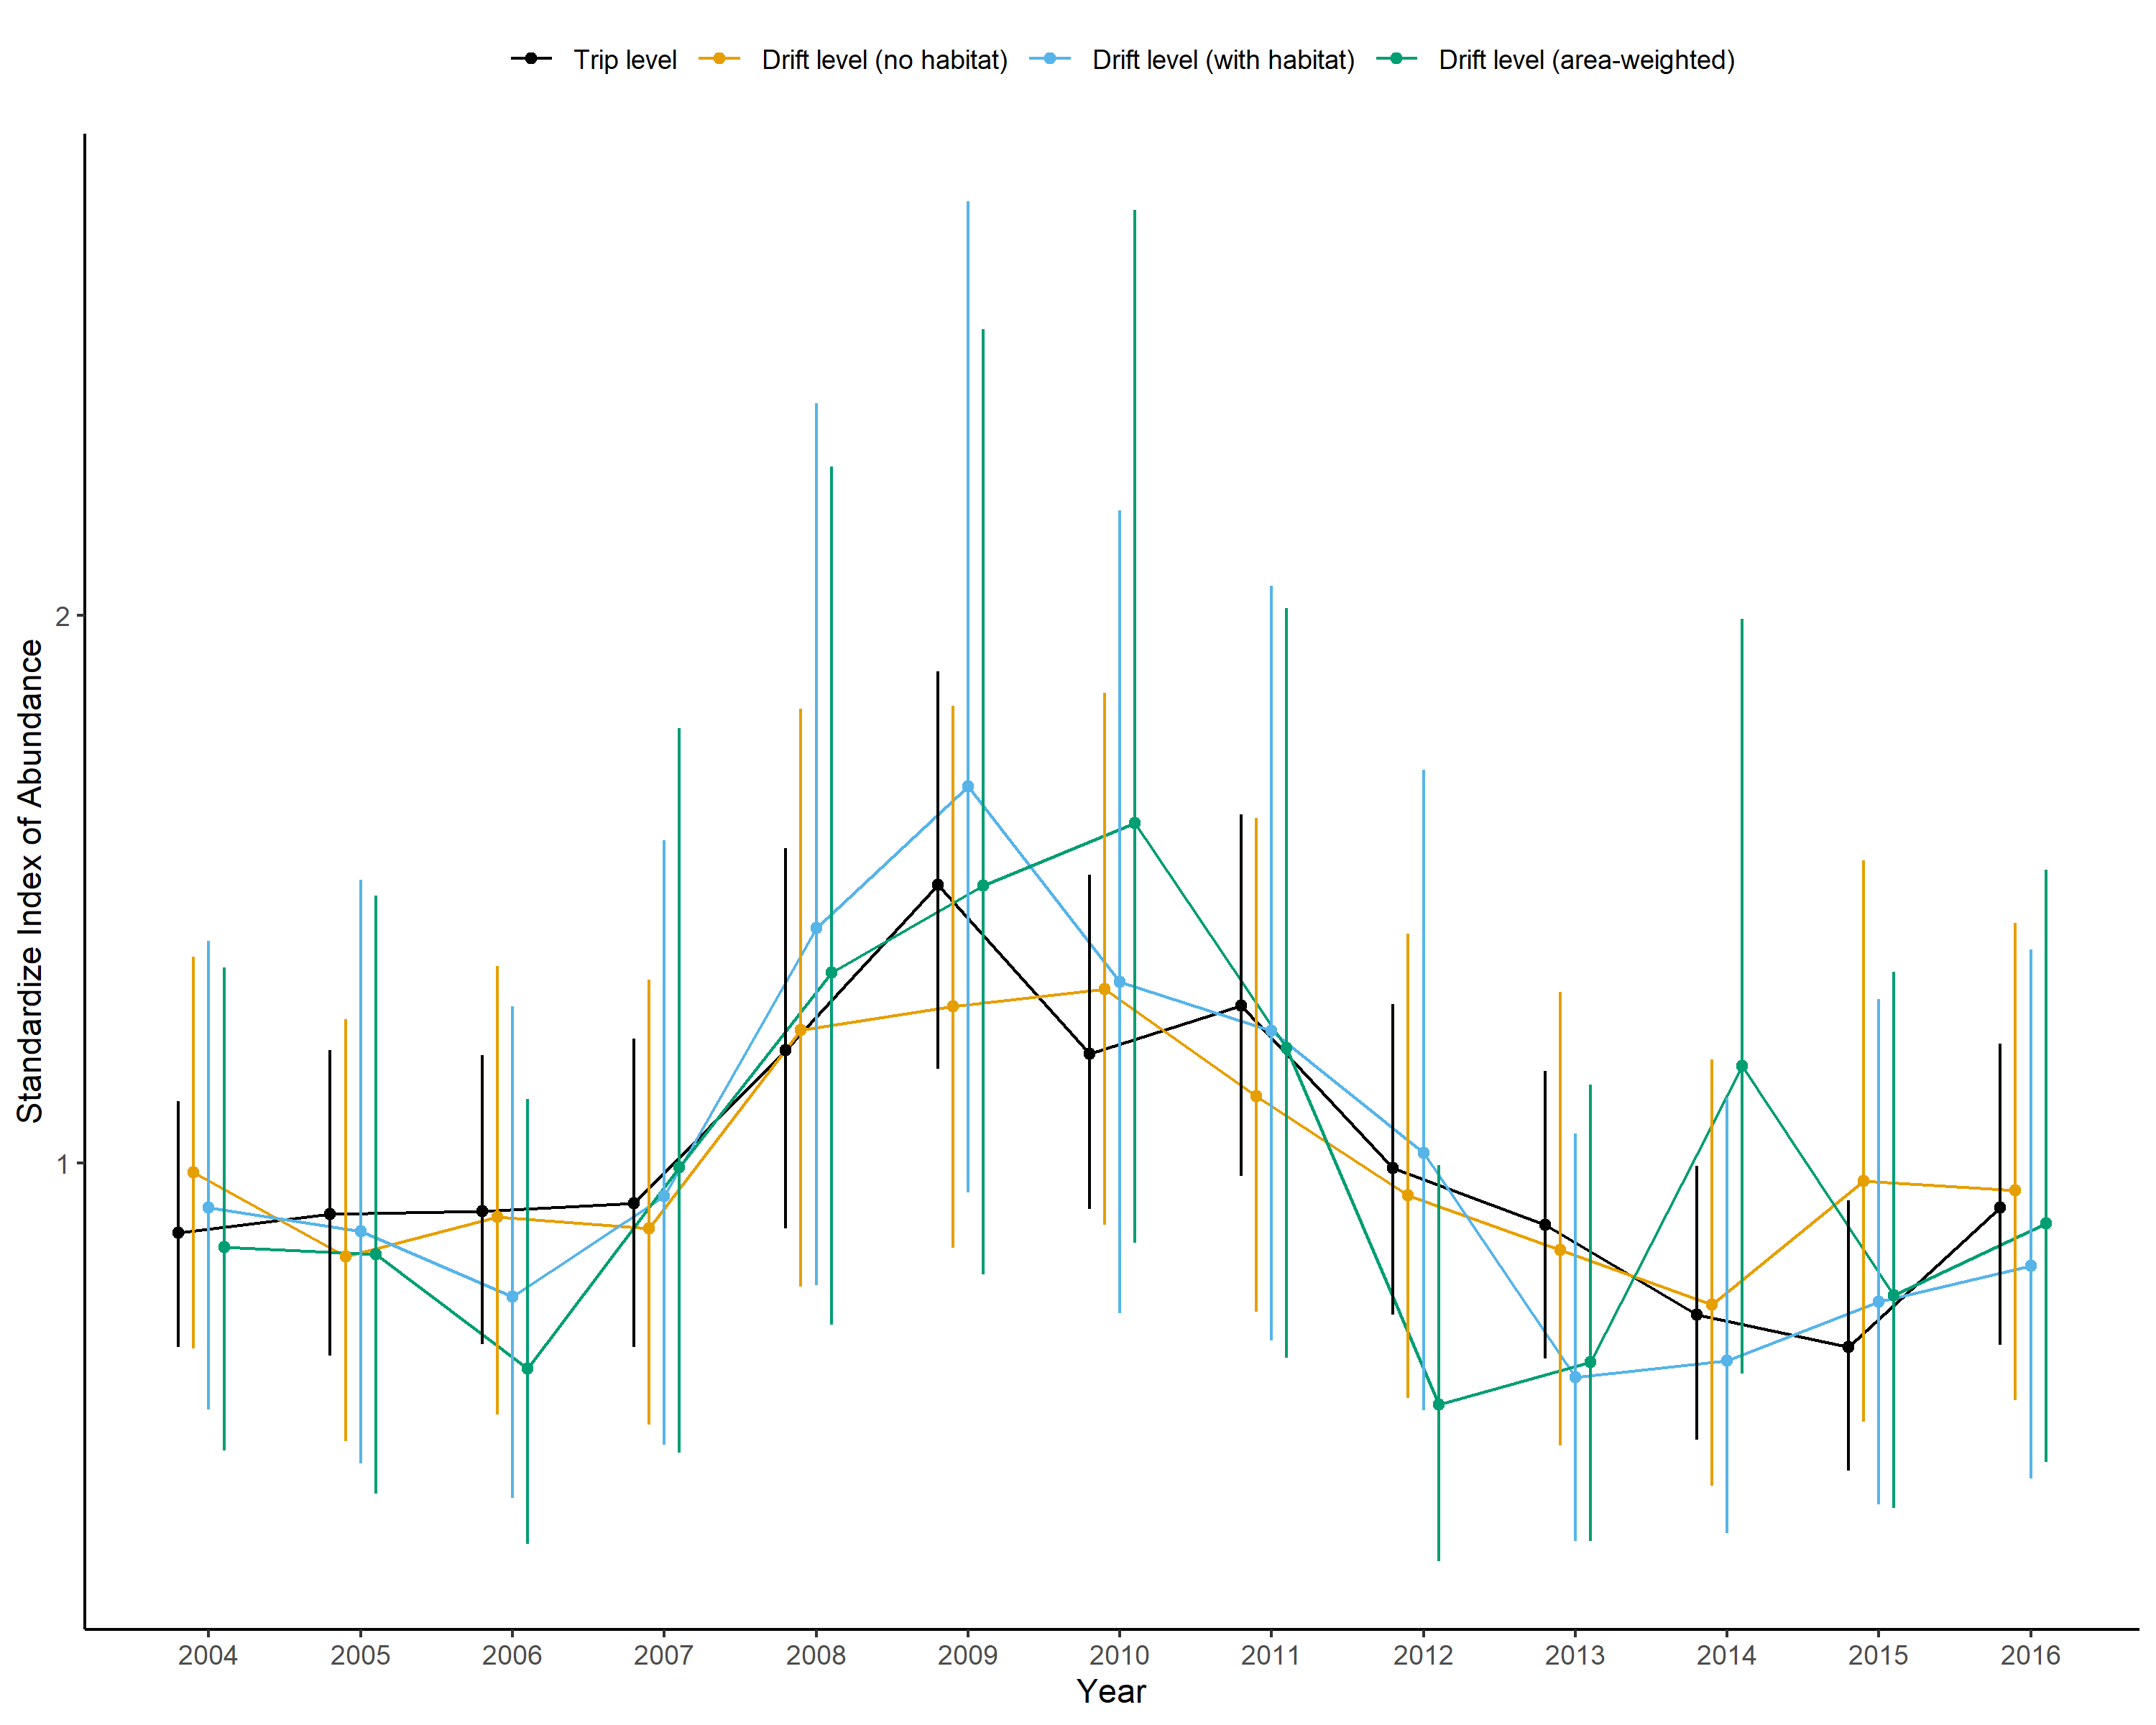
\includegraphics[width=3in,height=\textheight]{figures/china_indices.png}

}

}

\subcaption{\label{fig-china-indices}China rockfish}
\end{minipage}%
\newline
\begin{minipage}[t]{0.50\linewidth}

{\centering 

\raisebox{-\height}{

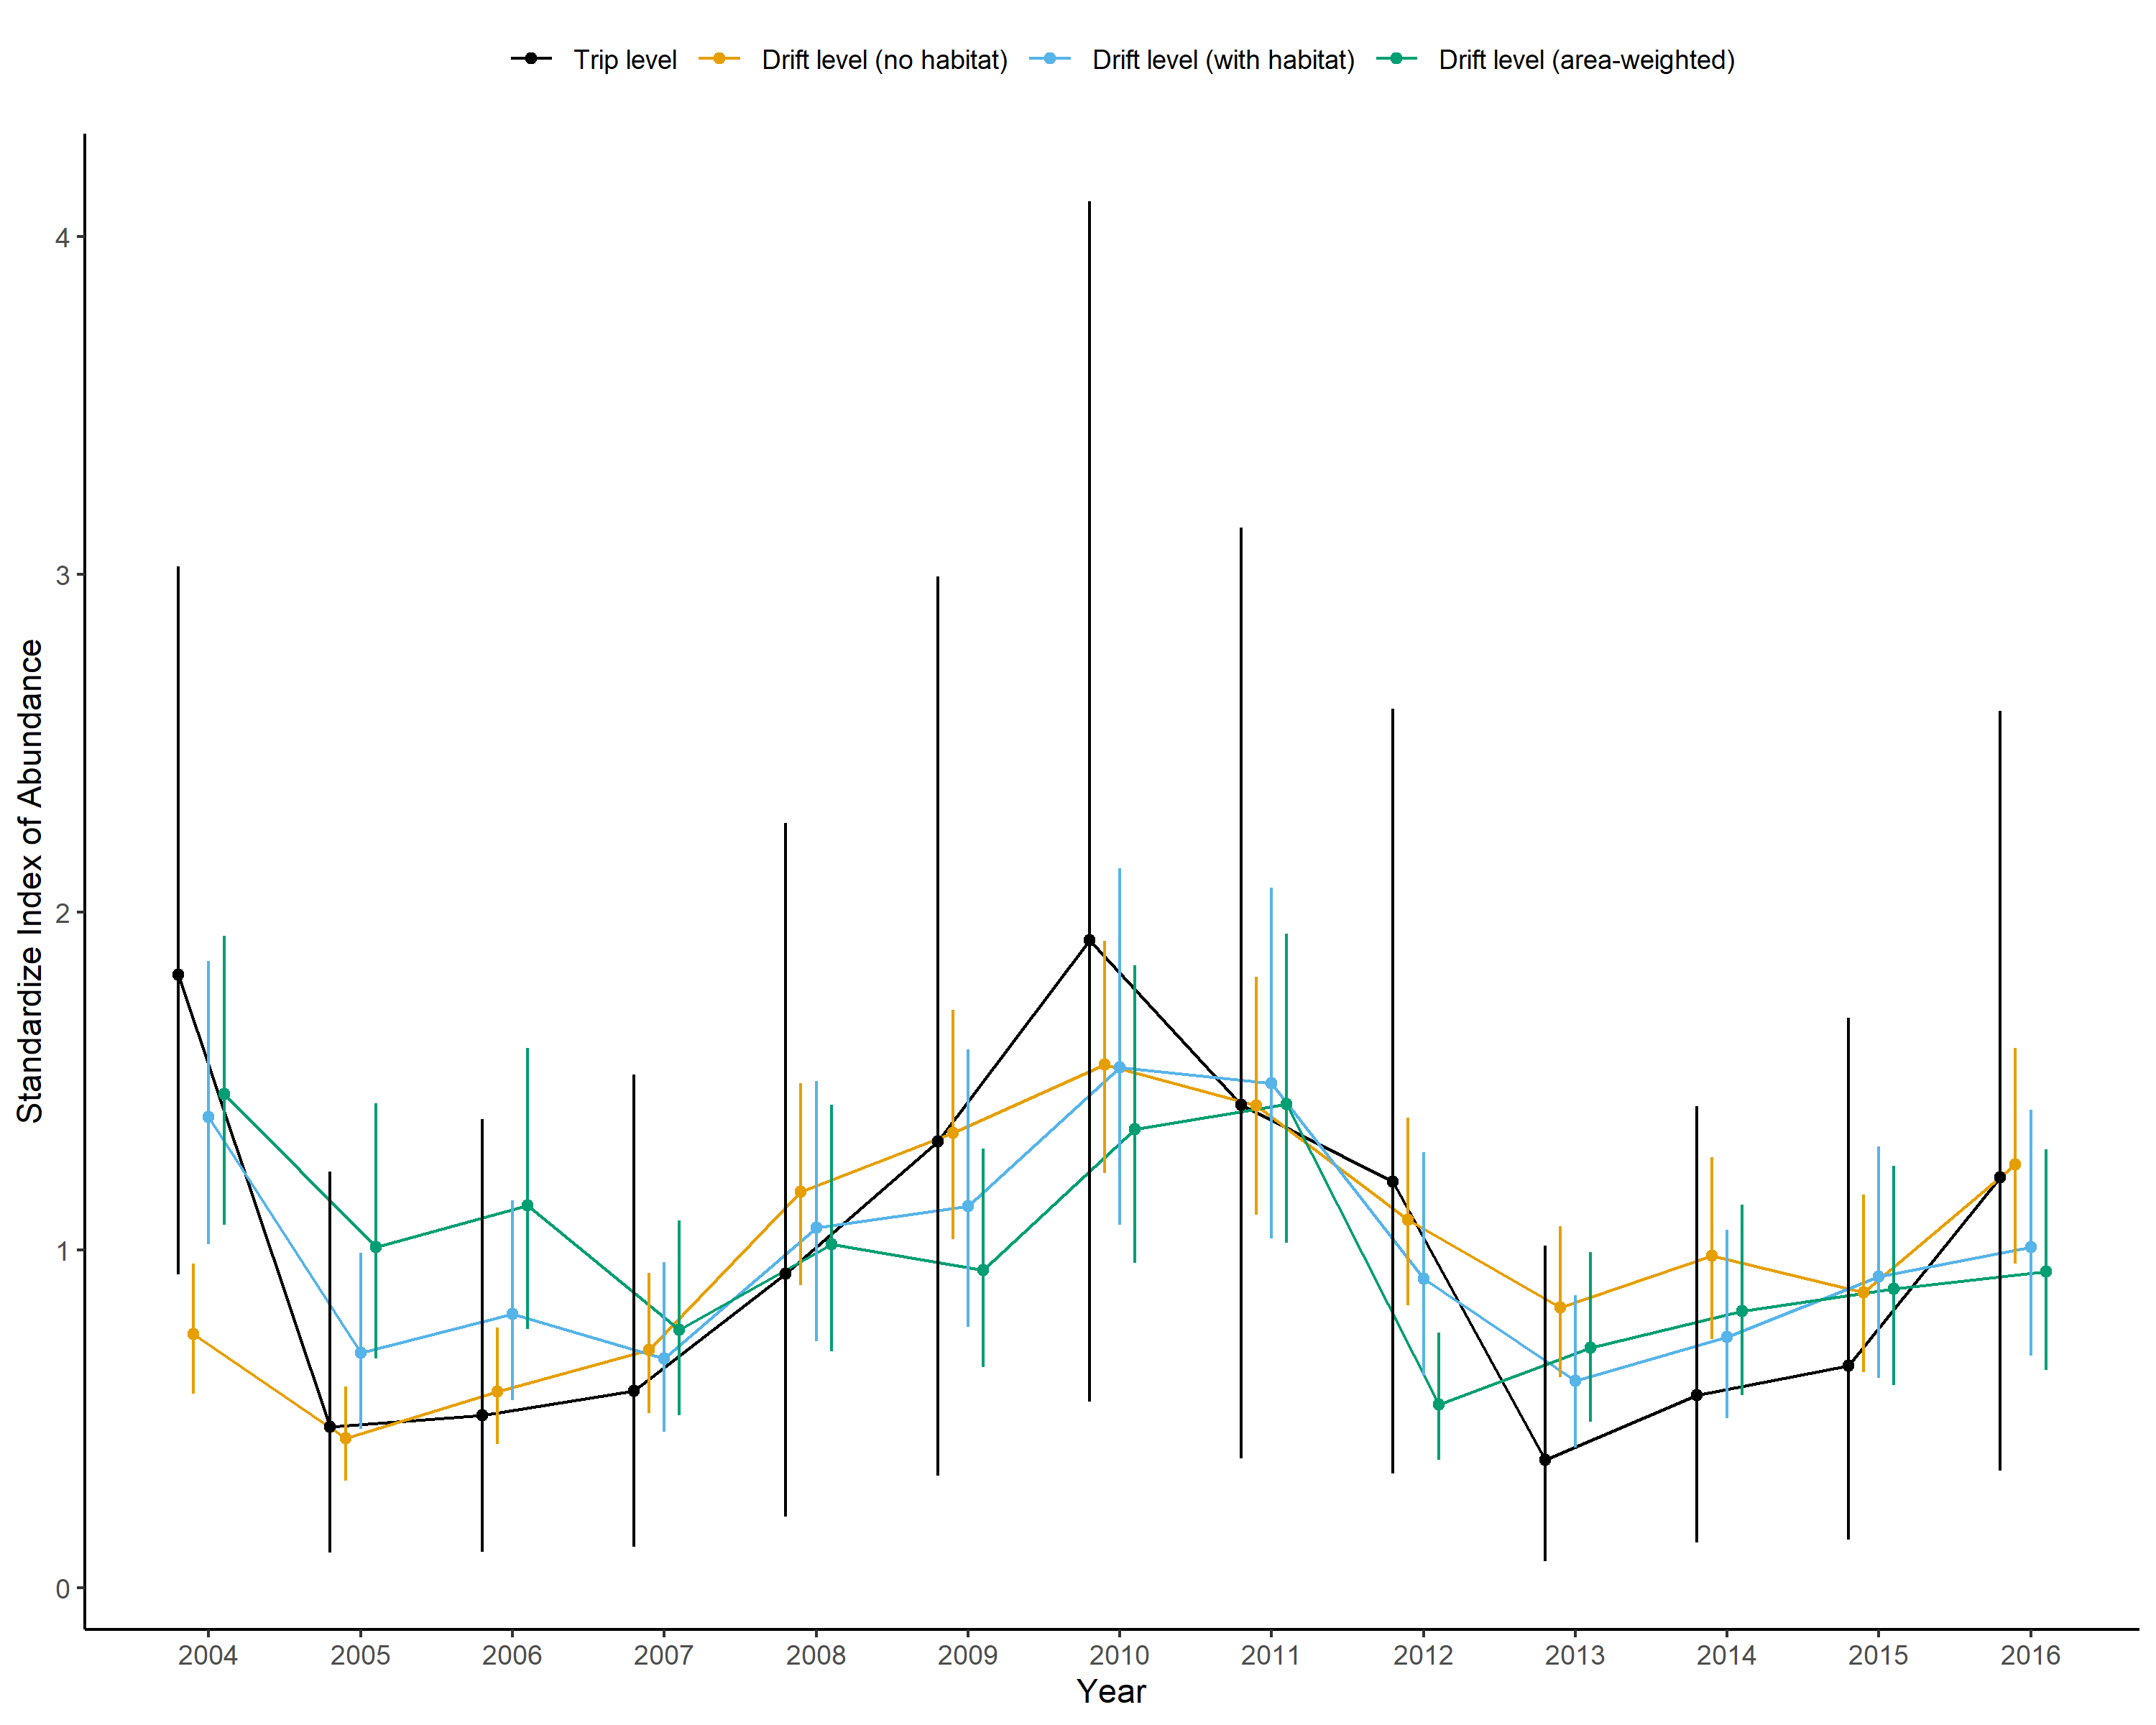
\includegraphics[width=3in,height=\textheight]{figures/gopher_indices.png}

}

}

\subcaption{\label{fig-gopher-indices}Gopher rockfish}
\end{minipage}%
%
\begin{minipage}[t]{0.50\linewidth}

{\centering 

\raisebox{-\height}{

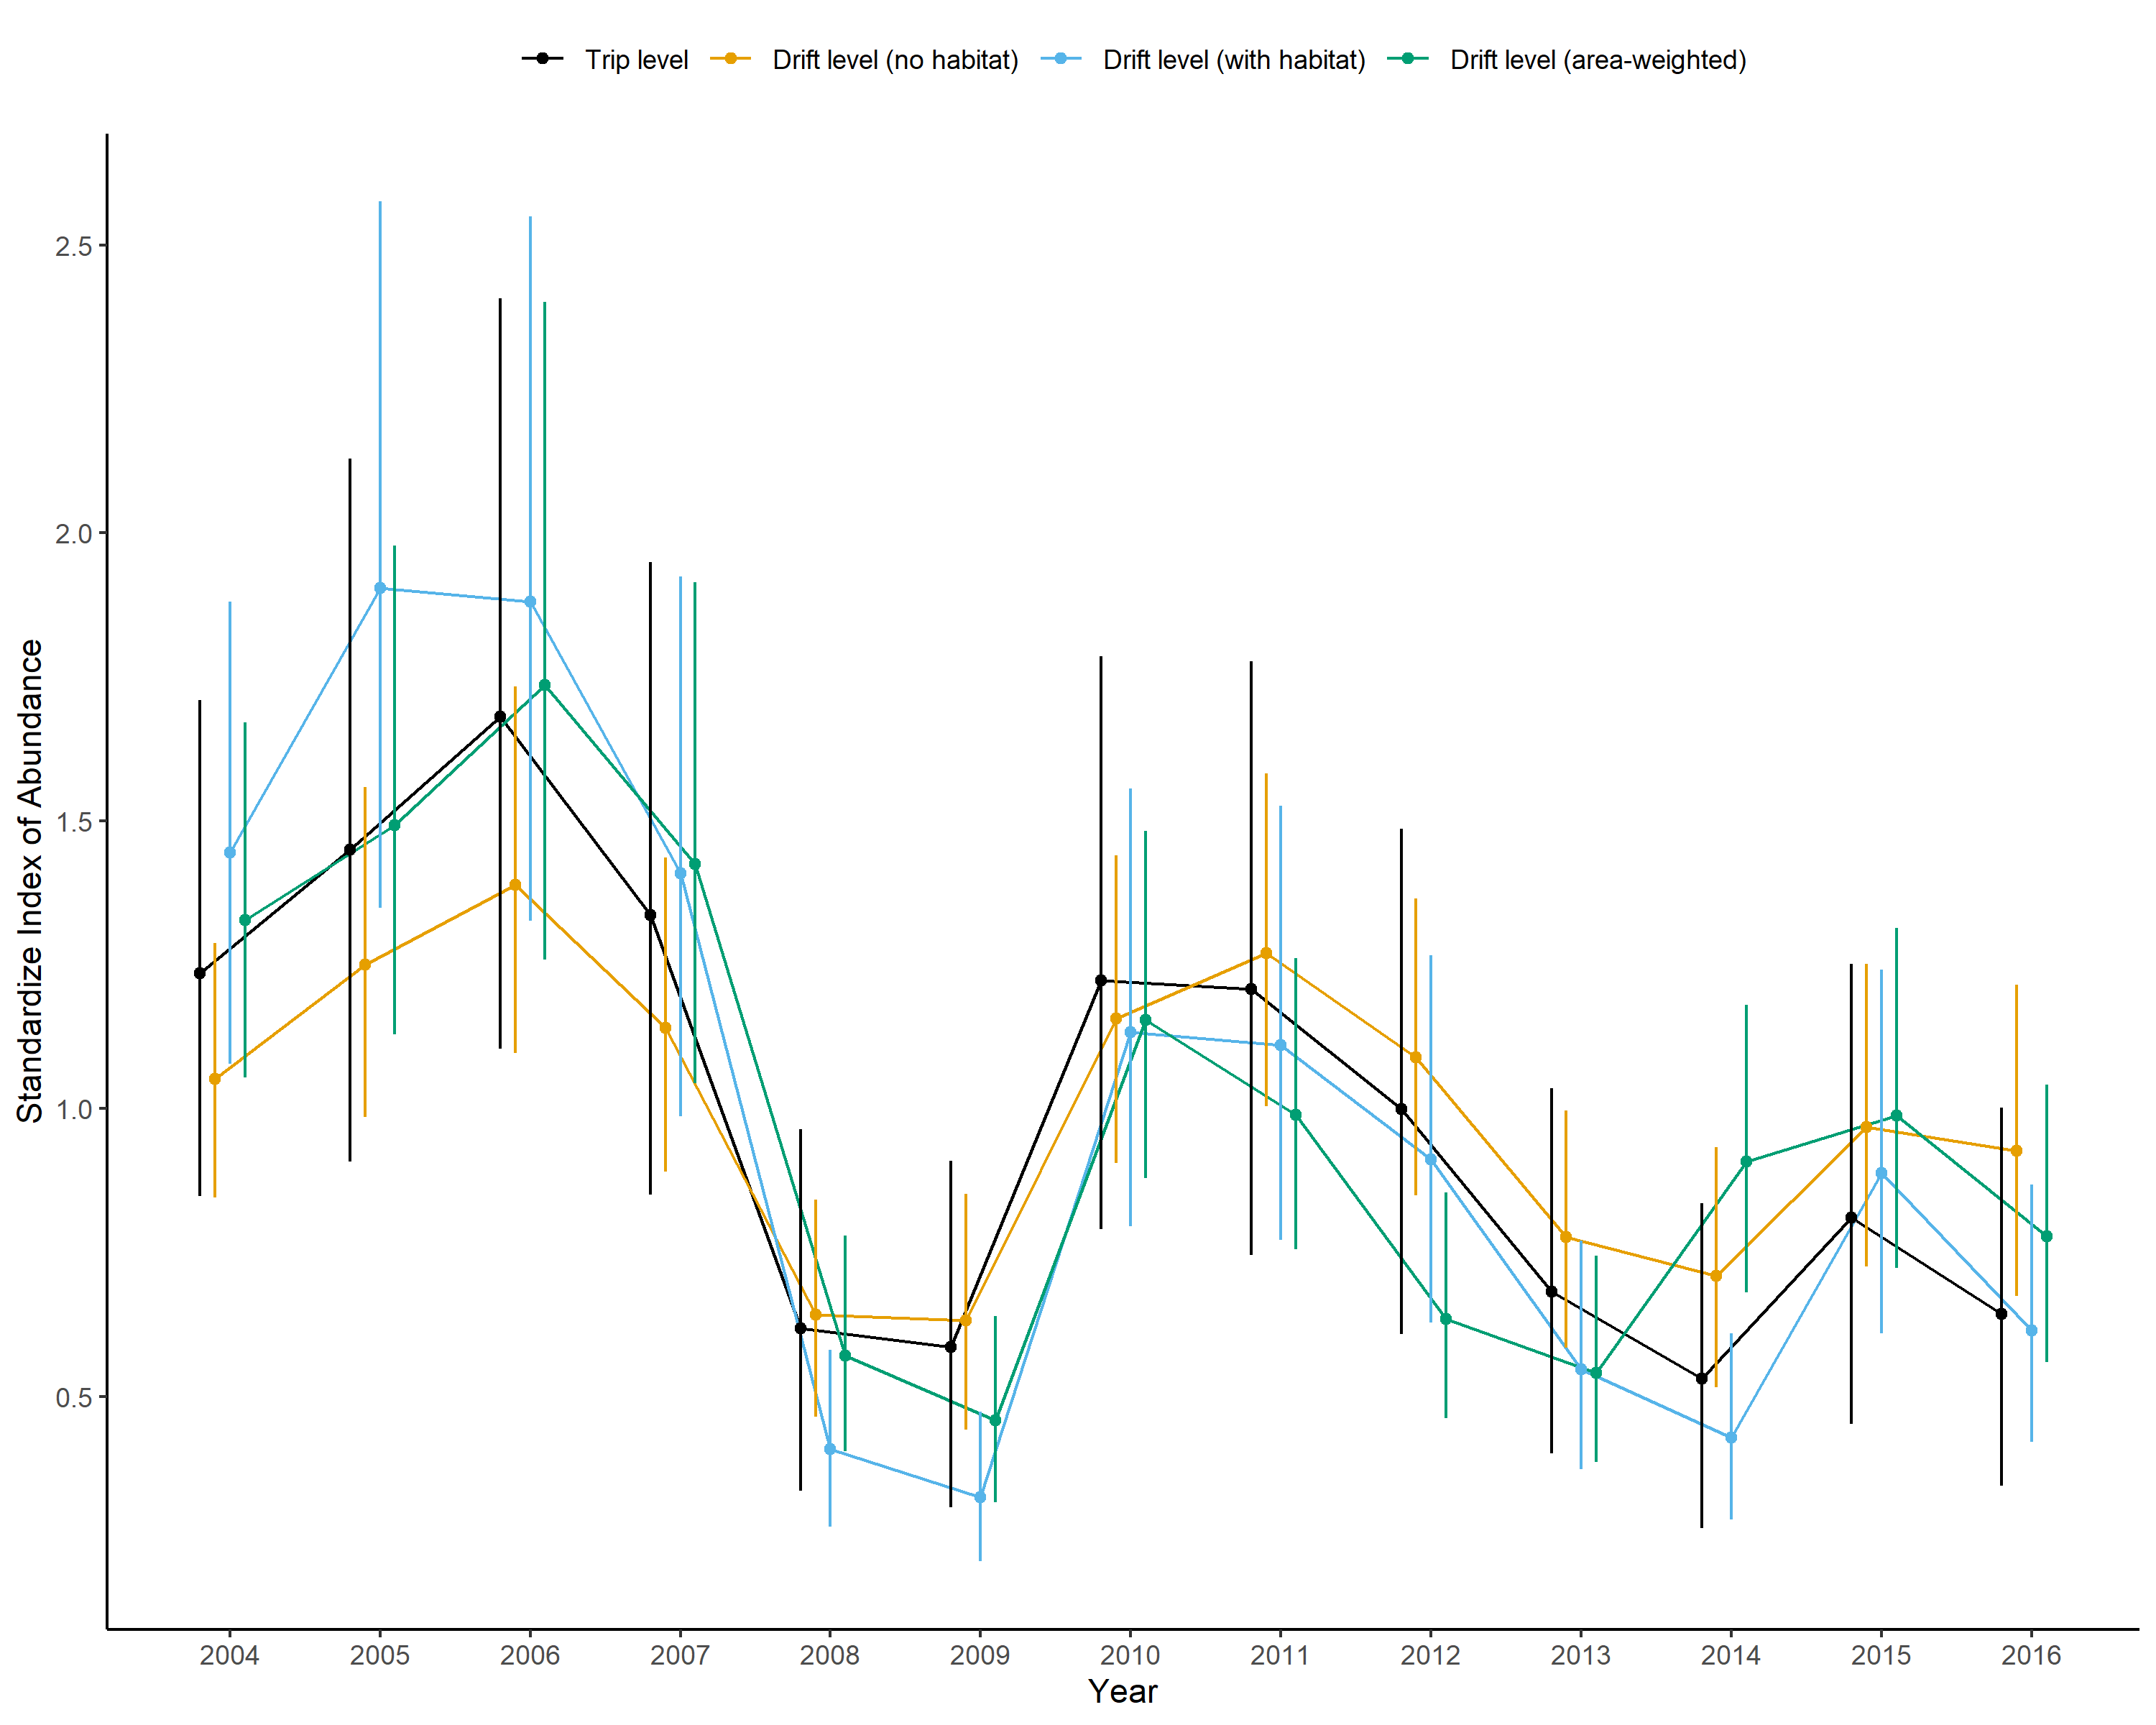
\includegraphics[width=3in,height=\textheight]{figures/vermilion_indices.png}

}

}

\subcaption{\label{fig-vermilion-indices}Vermilion rockfish}
\end{minipage}%

\caption{\label{fig-indices}Indices of abundance and 95\% confidence
intervals for the different filtering strategies, each scaled to its
mean, for the six species.}

\end{figure}

\FloatBarrier


  \bibliography{bibliography.bib}


\end{document}
